% define document
\documentclass[
	a4paper, 
	11.5pt,
	headings=small, 
	twoside, 
	titlepage=firstiscover, 
 	pagesize=auto,
  	version=last,
	open=any,
	BCOR=14mm,
  	chapterprefix=false]{scrbook}
\setkomafont{sectioning}{\rmfamily}
\usepackage{bookman}
\usepackage{gitfile-info}
\KOMAoptions{DIV=14}

% include all the preambel stuff, loaded packages, command definitions etc.
\usepackage{hk40preambel}

% provide pdf metadata
\hypersetup{
	pdftitle={Protocol - HessenKohorte, Neurology Department, Philipps-University Marburg},
	pdfsubject={Hessenkohorte Protocol},
	pdfauthor={PD Dr. med. David J. Pedrosa},
	pdfkeywords={Parkinson's disease, cohort study, hassia, quality-of-life}
}

% main document
\begin{document}
  \setstretch{1.5}
\chapter{Protocol}
\section{Introduction}
\subsection{Background}
Idiopathic Parkinson's disease (\acs{iPD})\acused{iPD} represents a chronic neurodegenerative disorder manifested by both motor and non-motor symptoms. The physical impairments in \ac{iPD} have a significant psychosocial impact and lead to considerable losses in patients'  \ac{QoL} and a high burden on (informal) caregivers. Several \ac{QoL} assessment tools have been developed so far, some of which are specific to \ac{iPD} \cite{stuhrenberg2022jpm}. However, none of the models take into account positive aspects of well-being or a subject's personal attitude (e.g., optimism) but also manifold aspects in someone's life such as lack of social support as possible stress factor or level of integration, to name a few. In the present project, an investigation of \ac{iPD}-patients' \ac{QoL} over time will be carried out. For this purpose, a longitudinal assessment using established and validated \ac{HRQOL}-questionnaires will be performed. In addition, holistic observations will be collected using the the \textsc{CHAPO}-model \cite{thieken2022jpd} -- an approach originally developed for the assessment of life quality of very old people\footnote{\url{https://ceres.uni-koeln.de/forschung/nrw80}} which will be adapted to aspects of \ac{iPD}-patients for this cohort study. The aim of this project is thus to record \ac{QoL} in a standardised way over a long period of time. This data will be additionally put into context to biomarkers obtained annually in form of a cranial \ac{MRI} and  blood, saliva, urine, hair and stool samples. We aim for the identification of biomedical markers with predictive value for \ac{QoL} changes. In addition, the approach in this longitudinal study also aims at ascertaining the support services needed to better address the needs of family members of \ac{iPD}-patients. Stress experience, changes in sleep patterns and \ac{QoL} losses over the observation period will be included in the analysis of caregivers to identify a surrogate for adequate support.

\subsection{Geographic context}
\ac{iPD} is one of the most common neurological diseases. Estimates put the incidence of the disease in Germany at \SI{84.1}{} per \num[round-precision = 0, round-mode = places]{100000}{} people and per year and assume a number of approx. \num[round-precision = 0, round-mode = places]{400000}{} people \cite{nerius2017parkinson}. In order to understand the special features of the \UKGM as far as the care of \ac{iPD} patients is concerned, it is necessary to know the location of Marburg. Approximately \SI[round-precision = 0, round-mode=places]{77000}{} people live in the city of Marburg which is located in the countryside of the centre of Germany. It is a university town and a district town in the federal state of Hesse (cf. Figure \ref{fig1:hesseGermany}). Due to its location at about \SI{80}{\km} direct distance between the metropolitan areas of Frankfurt am Main and Kassel, the role of the \UKGM must be understood as the predominant centre for medical care in the district. About \num[round-precision = 0, round-mode = places]{1500}{} people with \ac{iPD} are treated there every year. To ensure access to care for patients in the district of Marburg, the \ac{PANAMA} was founded in 2016 by the Neurology Department. In this care network, different actors work together to facilitate the integration of care services and improve outcomes for patients. At the same time, it is a tertiary centre that combines established treatment services for each stage of the disease with university medicine and offers a series of studies that can provide innovative forms of therapy. This makes it possible to offer modern and tailor-made therapy to people from beyond the region.

\begin{wrapfigure}{r}{0.45\textwidth} %this figure will be at the right
    \label{fig1:hesseGermany}
    \centering
    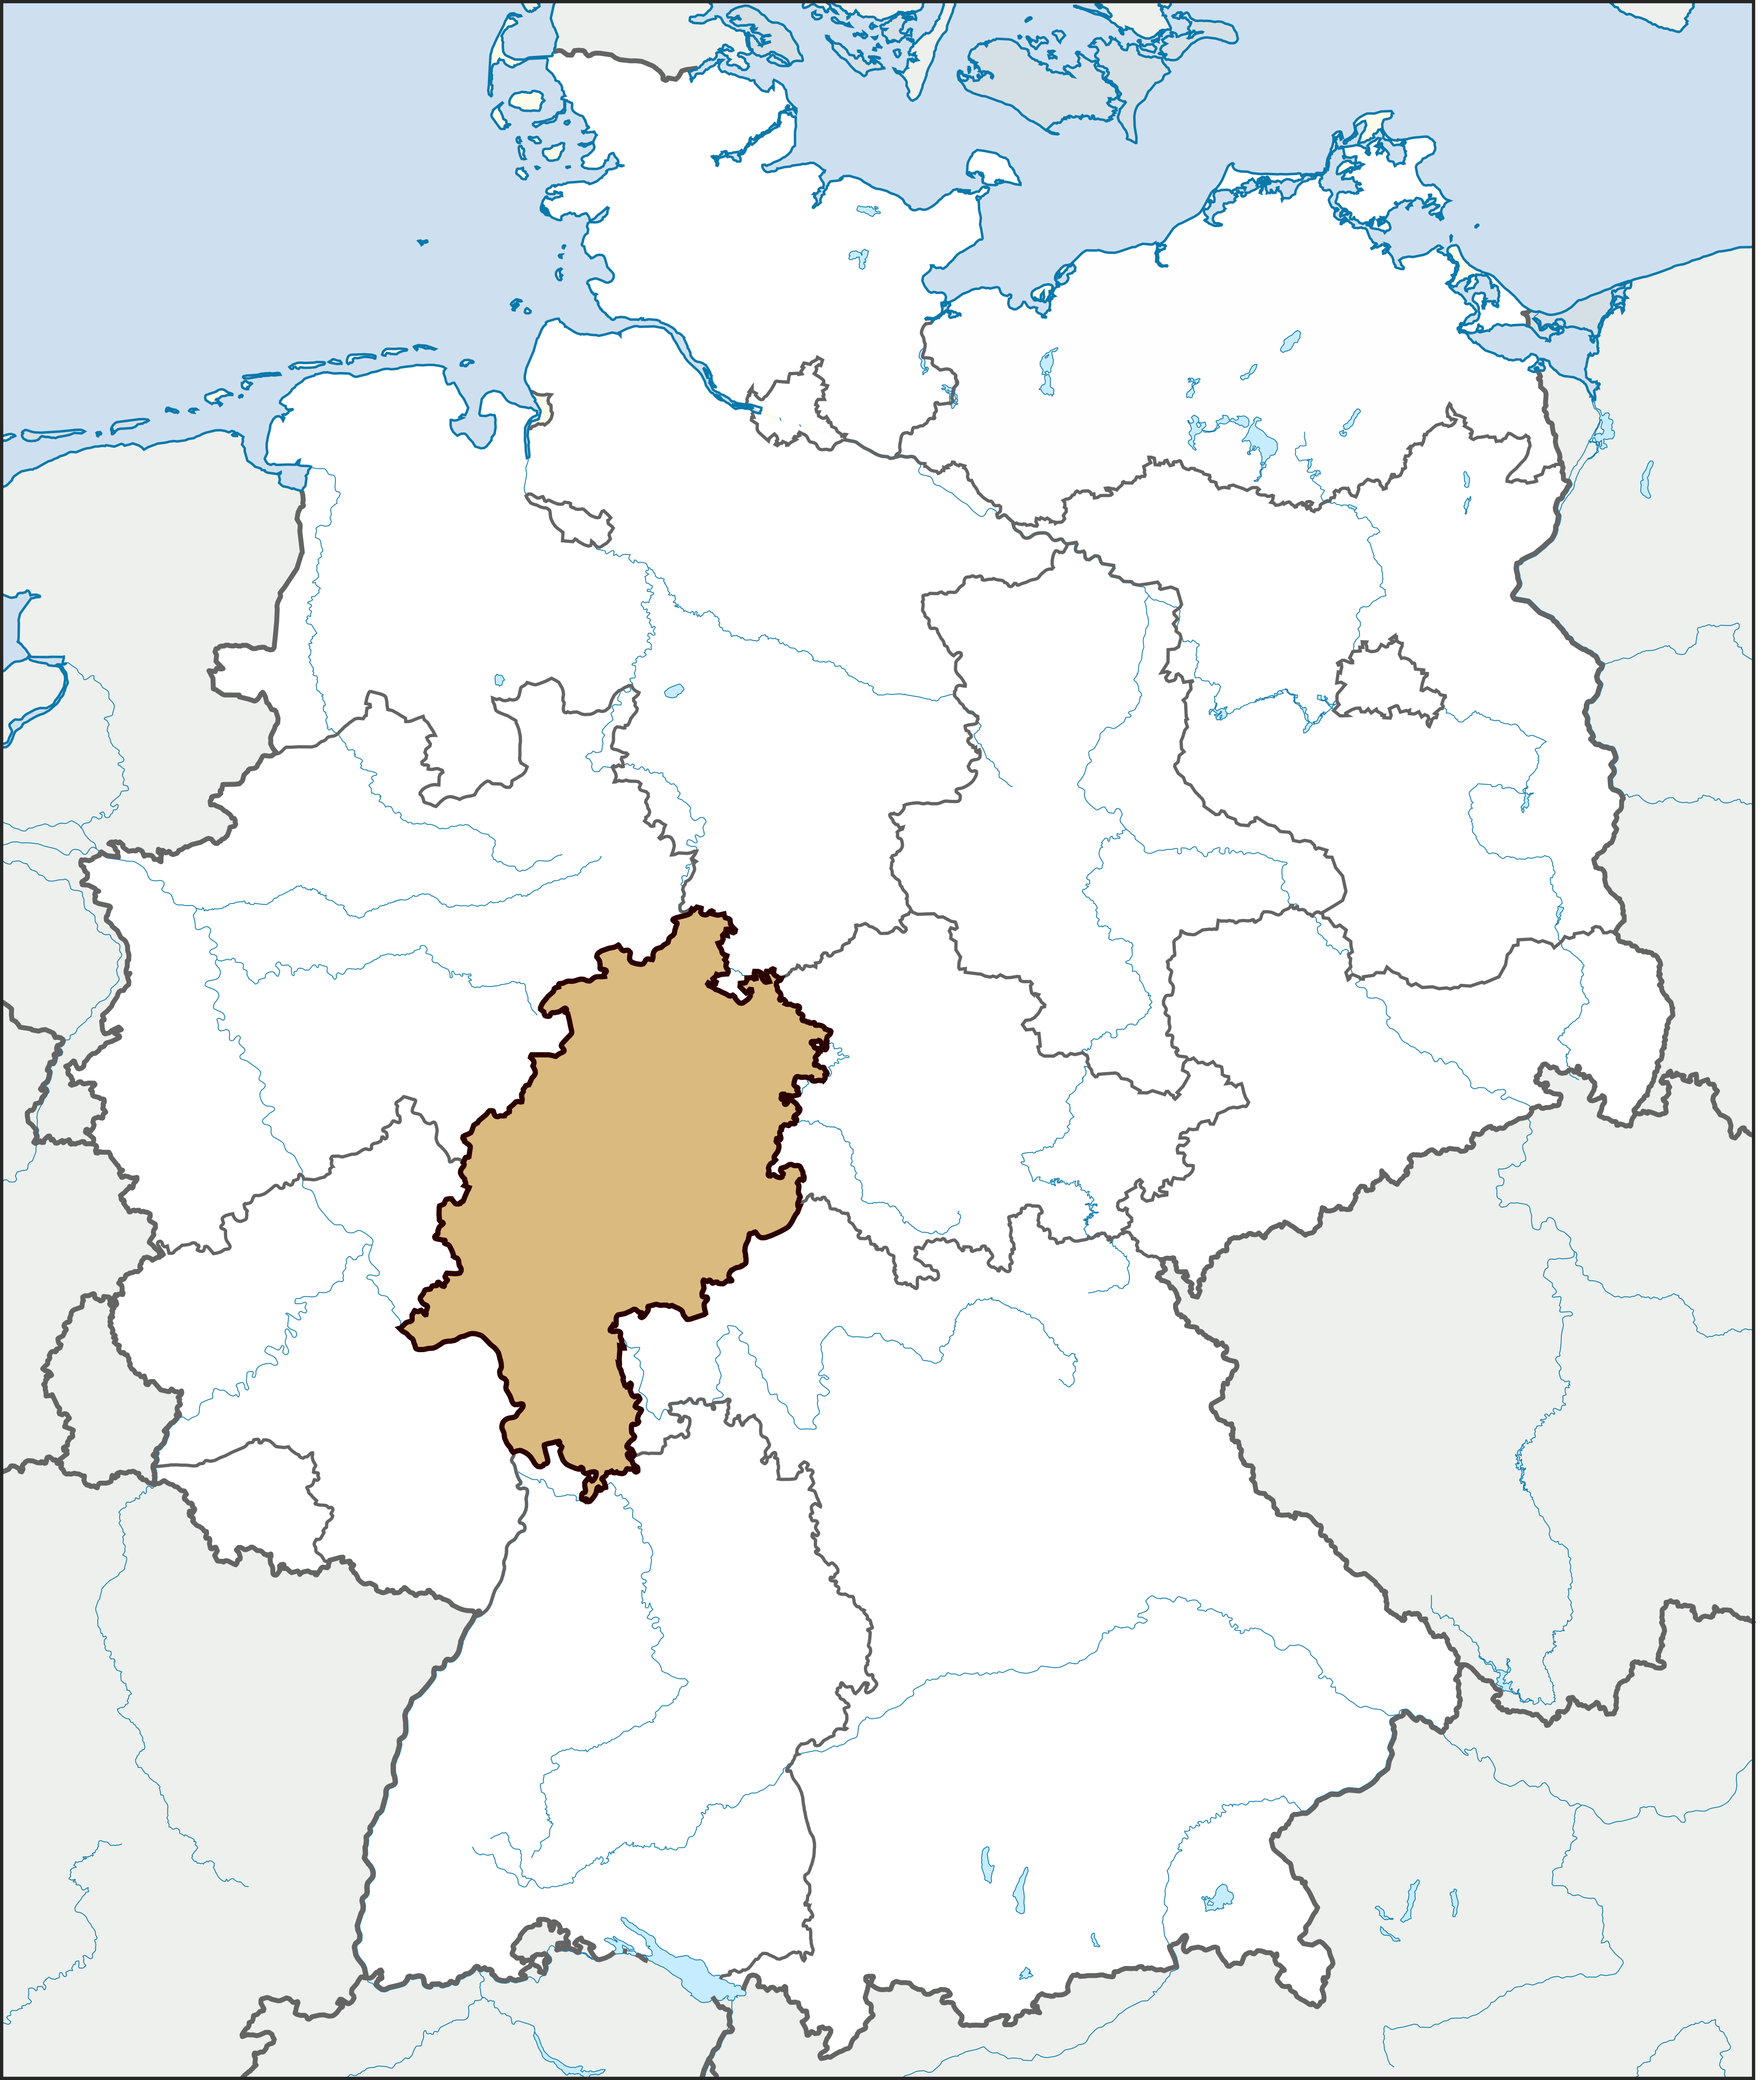
\includegraphics[width=0.45\textwidth]{Hesse_in_Germany.v1.0}
    \caption{Location of Hesse in the German Federal Republic}
\end{wrapfigure}

In order to represent the diversity of the population of \ac{iPD}-patients at \UKGM and to ensure a balanced study cohort, as many of the treated patients as possible should be given the opportunity to participate in the \textsc{HessenKohorte}. Accordingly, the management of the study will adopt the recruitment strategies that have been successfully tested in previous clinical studies and to adapt them to the requirements of the long-term cohort study. To this end, on the one hand, patients are directly offered participation in the study during their appointments in the outpatient clinic of the hospital or during their inpatient stay in the Neurology Department. Secondly, members of \ac{PANAMA} will be made aware of the study with the aim of arousing the interest of potential participants. Finally, detailed information will be made available on the media website of \UKGM to ensure sufficient information (\url{https://www.uni-marburg.de}).
\newpage

%%%%%%%%%%%%%%%%%%%%%%%%%%%%%%%%%%%%%%%%%%%%%%%%%%%%%%%%%%%%%%%%%%%%%%%
%%%% 										START OF SYNOPSIS												%%%%
%%%%%%%%%%%%%%%%%%%%%%%%%%%%%%%%%%%%%%%%%%%%%%%%%%%%%%%%%%%%%%%%%%%%%%%

\setstretch{1}
\section{Protocol synopsis}
\begin{tabularx}{1\textwidth}{m{3.5cm} | X}
\toprule
%\multicolumn{2}{c}{}\\
\multicolumn{2}{p{\dimexpr\linewidth-2\tabcolsep-2\arrayrulewidth}|}
{\textbf{
 Longitudinal digital observation of the holistic quality of the life of patients with \acl{iPD} and their caregivers: a prospective observational cohort study
}}
\\ \toprule

\textbf{Study objectives} & 
This study aims at observing \ac{QoL} of \num[round-precision = 0, round-mode = places]{1000} patients suffering from \ac{iPD} and their relatives over the course of 20 years and relating this to objectifiable changes in the metabolism but also to structural imaging changes during this time.
\\ \midrule

\textbf{Study design} &
Prospective single-center observational cohort study
\\ \midrule

\textbf{Planned Number of Subjects} &
\num[round-precision = 0, round-mode = places]{1000} 
\\ \midrule

\textbf{Primary Endpoint} &
Quality of life of the index patient after an observation of up to 20 years
\\ \midrule

\textbf{Secondary Endpoints} & 
\tabitem{Quality of life of the relatives of patients after an observation of up to 20 years} \\
& \tabitem{Changes in motor symptoms of the index patient after up to 20 years} \\
& \tabitem{Development of non-motor symptoms over up to 20 years} \\
& \tabitem{Changes of the functional imaging over the observational period} 
\\ \midrule

\textbf{Enrollment of participants} & Patients suffering from \ac{iPD} may be enrolled together with their relatives at any point in time.
\\ \midrule

\textbf{Study visits schedule} & 
\tabitem{Screening}\\
& \tabitem{Baseline Visit}\\
& \tabitem{Half annual visit}
& \tabitem{Annual visit}\\
& \tabitem{Unscheduled visits}\\
%& \tabitem{Visit at year 2042 (\textit{End-of-Study}-visit)}
% @David: wuerde ich weglassen. da machen wir ja nix spezielles und er
% kommt im ganzen restlichen Dokument (in den ganzen Tabellen und so)
% nicht mehr  vor
\\ \midrule 

\textbf{Study Duration} &
The study will be considered complete after all subjects complete their visit in the year 2043. Hence, the total study duration is estimated to be at most 20 years.
\\ \midrule

\textbf{Inclusion criteria \ac{iPD}-patients} &
\tabitem{Patients suffering from a clinical diagnosis of \acs{iPD} according to the recent clinical diagnostic criteria \cite{postuma2015mds}} \\
& \tabitem{\ac{iPD}-stages of \RNum{1} -- \RNum{4} according to the Hoehn \& Yahr
  scale (in the OFF state, i.e., without medication) \cite{hoehn1967parkinsonism}} \\
& \tabitem{Patients aged between between 30 and 100 years}\\
& \tabitem{Patients with the ability to provide informed consent. In
  cases where participants lose their capacity to consent at follow-up
  visits (e.g., due to dementia, etc.), this participant will only be
  allowed to continue if a legal representative (proxy, guardian)
  provides informed consent to further participation on behalf of the
  participant. In this case, the legal representatives will be
  provided with a separate consent form.} \\
% @David gibt es dieses spezielle form eigentlich?  
\\ \midrule

\textbf{Exclusion criteria \ac{iPD}-patients} &
\tabitem{Patients suffering from a clinical diagnosis of atypical 
  Parkinson's syndrome in a first instance. Patients enrolled who
  were later characterized as atypical Parkinson syndroms will not be
  excluded.}\\
& \tabitem{\ac{iPD}-stages of \RNum{5} according to the Hoehn \& Yahr scale
  (in the OFF stage, i.e. without medication) \cite{hoehn1967parkinsonism}}\\
& \tabitem{The use of magnetic fields in the MRI examination excludes
  the participation of persons who have electrical devices
  (e.g., cardiac pacemakers, medication pumps, etc.) or metal parts
  (e.g., screws after bone fracture) in or on their bodies.} \\
% wollen wir die wirklich gar nicht einschliessen (klingt so) oder
% bekommen die nur kein MRT?
& \tabitem{Women who are pregnant will not receive \ac{MRI}.} \\
& \tabitem{Subjects who do not want to be informed about possible
  incidental findings are also not allowed to participate in the
  imaging part of the study.}
  % finde ich immer noch etwas seltsam. ist das so ueblich?
\\ \midrule

\textbf{Inclusion criteria \ac{iPD}-patients' relatives} &
\tabitem{Relatives of patients included in the study according to the abovementioned criteria} \\
& \tabitem{Subjects with the ability to give informed consent} \\
\\ \midrule

\textbf{Exclusion criteria \ac{iPD}-patients' relatives} &
Relatives who are unable to give informed consent cannot participate in the study
\\ \midrule

\textbf{Statistical methods} &
Due to a large number of possible primary endpoints for consideration, a multitude of analyses will be conducted to examine changes and variability over the 20 years. Analyses will include logistic, linear, and non-linear models for assessing these data, among others. Primary interest will focus on established and longterm measures of quality-of-life (such as the \ac{PDQ39}\cite{jenkinson1997pdq39}) but also of clinical severity such as the \ac{MDS-UPDRS}\cite{goetz2007updrs}. For the secondary endpoints, clinical, imaging and biological verification studies on promising biological markers in study subsets using stored collected samples will be performed. These analyses may vary substantially depending on the type of marker and the data available.
\\ \midrule

\textbf{Statistical test method} & 
According to the primary endpoint and the envisaged number of participants, \ac{ANOVA} will be conducted in order to determine the predictors of decreases in \ac{QoL} during the \ac{iPD}-patients' course. Furthermore, studies correlating \ac{QoL} to the identified markers and results in imaging should be performed.
% ist vielleicht nicht so wichtig aber wie saehe das ANOVA hier modell aus?
\\ \midrule

\textbf{Sample Size Parameters} & 
This is a longitudinal cohort study where the number of participants is determined by the number of resources available. The number of participants is therefore composed of the expected number of patients in the district and the resources available to the centre (\UKGM{}).
\\ \bottomrule
\end{tabularx}
\newpage

%%%%%%%%%%%%%%%%%%%%%%%%%%%%%%%%%%%%%%%%%%%%%%%%%%%%%%%%%%%%%%%%%%%%%%%
%%%% 										END OF SYNOPSIS													%%%%
%%%%%%%%%%%%%%%%%%%%%%%%%%%%%%%%%%%%%%%%%%%%%%%%%%%%%%%%%%%%%%%%%%%%%%%

\setstretch{1.5}
\section{Study objectives and endpoints}
\subsection{Study objectives}
The primary aim of the \textsc{HessenKohorte} is to deepen the understanding of the development of \ac{QoL} in \ac{iPD}-patients and to identify factors with favourable or detrimental impact thereon in an representative German cohort. Furthermore, the study aims at improving our understanding of the diseases' impact on the caregivers and to find out which factors or forms of structural support make these family caregivers more resilient to those burdens resulting while caring for a person with \ac{iPD}.
% (wie) erheben wir denn den 'structural support'? 

\subsection{Primary study endpoint}
The primary endpoint of the \textsc{HessenKohorte} is the index patients' \ac{QoL}. For that, a model was developed which measures not only the disease related aspects of life quality (\ac{CHAPO-PD}) but also additional factors which foster \ac{QoL} and thus go beyond healthcare-related issues. This will be ascertained along with established questionnaires such as the \ac{PDQ39}\cite{jenkinson1997pdq39}, or the \ac{WHOQoL}\cite{group1998world} and may be related to other characteristics of included patients.

\subsection{Secondary study endpoint}
According to the large number of possible analyses and secondary endpoints for consideration, the authors foresee a substantial
number of analyses to be conducted in order to contemplate changes over time. Yet, a list of a few possible secondary endpoints shall be named:
\begin{itemize}
  \item{Changes in motor symptoms of the index patient after up to 20 years}
  \item{Development of non-motor symptoms over up to 20 years}
  \item{Changes of the structural imaging over the observational period} 
\end{itemize}
Irrespective of the unique characteristics of a study on \ac{QoL} of people with \ac{iPD}, standard examinations of \ac{iPD}-patients should also be carried out as far as the secondary endpoints are concerned. At this point, motor along with non-motor symptoms should be mentioned as the most common symptoms encountered. The former constitute the hallmark of the disease, whereas the latter are incresingly recognized as responsible for huge losses in \ac{QoL} (Quelle). The extent of motor symptoms will be operationalised via part III of the \ac{MDS-UPDRS}\cite{goetz2007updrs}. Non-motor symptoms will be measured using the \ac{NMSQ} a measure able to capture a wide variety of different aspects with regard to this symptom domain. An overview with the scheduled time points of all questionnaires can be found in table \ref{tab:questionnaireSchedule}.

\section{Study design}
The \textsc{HessenKohorte} is a longitudinal, observational, natural history study to assess \ac{QoL} progression in study participants suffering from \ac{iPD}. The intended cohort size of \num[round-precision = 0, round-mode = places]{1000}{} will be comprehensively assessed for a maximum of five years. All subjects along with their relatives will undergo clinical assessments (motor, non-motor, cognitive neuropsychiatric and \ac{QoL}) and imaging assessments, and will be asked to donate biosamples including blood, urine, saliva, hair and stool. Participants will also be asked to respond to questionnaires and provide digital data as part of the \textsc{HessenKohorte}.
% was bedeutet der Teil mit den 5 Jahren?
% hier klingt es so, als würde wir die biosamples/MRT auch von den relatives erheben?

\subsection{Scale and duration}
The study will accompany up to \num[round-precision = 0, round-mode = places]{1000}{} patients over at most 20 years to enable a profound insight into the life course of patients' and relatives' \ac{QoL}.

\subsection{Justification for study design}
The \textsc{HessenKohorte} is a single-centre, longitudinal and observational follow-up assessment of \ac{iPD}-patients' \ac{QoL}. This unique primary endpoint will be assessed using a newly developed questionnaire, the main feature of which is a holistic assessment that looks not only at disease-related limitations but also at existing resources and the social environment of those affected \cite{thieken2022jpd}. Accordingly, the inclusion of relatives is fundamental to obtain effects of the disease on the patient's entire environment. The comparatively large number of subjects should provide a good insight into the lives of \ac{iPD}-patients with their multi-layered phenotypes, but also offer possibilities for diverse investigations through the additional recording of biosamples.

\subsection{Hypotheses}
\label{sec:hypoTheses}
The primary endpoint of the study is the development of \ac{iPD}-patients' \ac{QoL} over the course of up to 20 years. The \textsc{HessenKohorte} thereby addresses the following main scientific hypothesis:
\begin{itemize}
  \item Exploratory analysis of the development of \acl{QoL} over the course of the disease.
\end{itemize}
The design of the study is based on the currently accepted assumption that \ac{QoL} of \ac{iPD}-patients correlates significantly with symptom severity. It can also be assumed that the \ac{QoL} of those affected strongly relates to that of their relatives. The present study design is intended to contribute to longitudinal \ac{QoL} assessment, but especially to allow exploratory studies in the course of or at the end of data collection, which could provide information on whether certain factors in the behavioural data, the imaging or the biospecimens provided could have a predictive value.
% der letzte Satz klingt etwas hazy fuer mich. was ist da die Aussage?

\subsection{Planned analyses}
Our main method for assessing the hypotheses are \ac{ANOVA}, linear regression and correlation analyses. In particular we will analyse the correlation between the \ac{QoL} of the index patient and of her relatives and caregivers. In order to extend this analysis we will assess different influencing factors as e.g. age, gender and symptom burden (motor and non-motor). Furthermore in an attempt to elucidate the causal form of the interdependence we will analyse how \ac{QoL} of patients/caregivers at earlier timepoints relates to \ac{QoL} of caregivers/patients at a later point in time.

With regard to our hypothesis concerning the prediction of disease progress, we will primarily rely on linear and regression methods. We will try to offer models predicting disease symptoms at the end of the study compared to the status at earlier timepoints. While we first will look at a linear relationship we will also consider more complicated models when they are necessary to model disease progress convincingly. Also in this analysis mediating or moderating variables especially from sociodemographic data may play a role and will accordingly be considered.

\begin{figure}[h]
\label{fig2:scheme}
\centering
\includegraphics[width=1\textwidth]{Schema_HessenKohorte.v1.0}
\caption{Schematic overview of the planned analyses. Subjects will be enrolled subsequently and will receive regular follow-ups. In addition to clinical data in form of different questionnaires, biomarkers including cranial \ac{MRI}, blood, saliva, urine, hair and stool samples will be collected at an annual basis.}
\end{figure}


\section{Subject selection}
\label{sec:study_selection}
\subsection{Study population and Eligibility}
\label{sec:study_population}
Study candidates will be drawn from the patients treated in the Neurology Department of the \UKGM, Marburg site, as either in- or outpatients. Moreover, all patients in the federal state of Hesse suffering from \ac{iPD} may submit a request for participation in the study. The inclusion and exclusion criteria (cf. Section \ref{sec:inclusion_criteriaIPS}) are checked by one of the study physicians, who are responsible for the final decision. Advertising for the study can be found in the form of a flyer, which is available in the Department of Neurology, but also in the form of an internet homepage, where the project will be presented to the public and we will promote study participation over the \ac{PANAMA} network.

\subsection{Inclusion and exclusion criteria \ac{iPD}-patients}
\label{sec:inclusion_criteriaIPS}
Subjects who meet all the following inclusion criteria may be given consideration for inclusion in this cohort study, provided no exclusion criteria are met (for both, cf. table \ref{tab:inclusionexclusionCriteriaPatients}).

\begin{tabularx}{\textwidth}[!h]{X|X}
\caption{Inclusion and exclusion criteria for \ac{iPD}-patients to
  participate in the
  \textsc{HessenKohorte}}\label{tab:inclusionexclusionCriteriaPatients}\\ 
\toprule
\multicolumn{1}{c}{\textbf{inclusion criteria}} &
\multicolumn{1}{c}{\textbf{exclusion criteria}} \\ \toprule
\tabitem{Patients suffering from a clinical diagnosis of \ac{iPD}
  according to the recent clinical diagnostic criteria
  \cite{postuma2015mds}}

\tabitem{\ac{iPD}-stages of \RNum{1} -- \RNum{4} according to the Hoehn \& Yahr
  scale\cite{hoehn1967parkinsonism} (in the OFF stage, i.e., without
  medication)} \\

\tabitem{Patients aged between between 30 and 100 years}\\ % Amendment, dass auch Menschen ab 18 Jahren eingeschlossen werden können

\tabitem{Patients with the ability to provide informed consent. In
  cases where participants lose this capacity at follow-up visits
  (e.g., due to dementia, etc.), participants will only be allowed to
  continue if legal representative provides informed consent to
  further participation on hisor her behalf. In this case, the legal
  representative will be provided with a separate consent form
  \ref{einfügen}}
&
\tabitem{Patients suffering from a clinical diagnosis of atypical
  Parkinson's syndrome in a first instance. Patients enrolled who were
  later characterized as atypical Parkinson syndroms will not be
  excluded.}

\tabitem{\ac{iPD}-stages of V according to the Hoehn \& Yahr scale
  \cite{hoehn1967parkinsonism} (in the OFF stage, i.e. without
  medication)}

\tabitem{The use of magnetic fields in the \ac{MRI} examination
  excludes the participation of persons who have electrical devices
  (e.g., cardiac pacemakers, medication pumps, etc.) or metal parts
  (e.g. screws after bone fracture) in or on their bodies.}

\tabitem{Women who are pregnant will not receive \ac{MRI} scans.} 

\tabitem{Subjects who do not want to be informed about possible
  incidental findings are also not allowed to participate in the
  imaging part of the study.} \\ \bottomrule
\end{tabularx}


\subsection{Inclusion criteria \ac{iPD}-patients' relatives}
\label{sec:inclusion_criteriaREL}
Only if a patient is included, the relatives may be asked for participation in the study. Subjects who agree to take part in the \textsc{HessenKohorte} must meet all the following inclusion and exclusion criteria (cf. Table  \ref{tab:inclusionexclusionCriteriaRelatives}).

\begin{tabularx}{\textwidth}{X | X}
\caption{Inclusion and exclusion criteria for relatives of
  \ac{iPD}-patients to participate in the
  \textsc{HessenKohorte}}\label{tab:inclusionexclusionCriteriaRelatives}\\
\toprule
\multicolumn{1}{c}{\textbf{inclusion criteria}}
&
\multicolumn{1}{c}{\textbf{exclusion criteria}} \\
\toprule
\tabitem{Relatives of \ac{iPD}-patients included in the study
  according to the abovementioned criteria (cf. Table
  \ref{sec:inclusion_criteriaIPS})}
&
\tabitem{Relatives who are unable to give informed consent}

\tabitem{Relatives with the ability to give informed consent} \\
\bottomrule
\end{tabularx}


\section{Subject accountability}
\subsection{Point of enrollment}
Subject will be considered to be enrolled at the time of the study-specific \ac{ICF} execution. No study-related procedures or assessments can take place until the \ac{ICF} is signed.

\subsection{Withdrawal}
All enrolled subjects (including those who have dropped out) must be recorded and documented. In case participants drop out of the study, an end-of-study form (\ref{sec:EOSform}) must be filled out and asked for the reasons for dropping out. 
% TODO this (reasons) has to be implemented in the form yet

Reasons for withdrawal include but are not limited to:
\begin{itemize}
  \item subject or relative choice to withdraw consent
  \item lost to follow-up
  \item pregnancy\footnote{\label{note1} only MR-imaging will be discontinued during pregnancy or from the moment of an implantation onwards.}
  \item implantation of electrical devices or metal parts in or on the body\footref{note1}
\end{itemize}

Subjects may withdraw at any time, with or without reason, and without prejudice to further treatment. Applicable \ac{CRF} up to the point of subject withdrawal and an end-of-study form \ref{chap:appendix} must be completed. Any subject deemed lost to follow-up should have a minimum of three documented attempts to contact him/her prior to completion of the end-of-study form. Additional study data may no longer be collected after the point at which a subject has been withdrawn from the study or withdraws consent, independent of the reasons. Data collected up to the point of subject withdrawal may be used. Subjects withdrawn after completing the implant procedure will not be replaced.
% which 'implant procedure'?
%TODO: We need to draw and End-of-Study-Form @Steffi

\subsection{Lost to follow-up}
Patients who do not react to the invitation to fill ou the questionnaires will be contacted in total three times per mail or email:
\begin{itemize}
\item 30 days before the planned visit
\item at the date of the visit and
\item 30 days thereafter
\end{itemize}
 If there is no answer to the third contact attempt, patients will be contacted per telefone in order to find out if there is a problem. Patients who cannot be contacted will receive the same number of mails/calls one year and two years after. In case of three years without response, an end-of-study form (cf. \ref{}) will be filled out and the subject is excluded. Vacant places due to excluded subjects may be filled up 5 and 10 years after the onset of the study.
% warum 5 und 10  Jahre und nicht einfach kontinuierlich?

\subsection{Subject status and classification}
A subject will be considered enrolled in this study at the time of the study-specific \ac{ICF} execution.

\subsection{Enrolment control}
The overall enrollment in the study will be capped at \num[round-precision = 0, round-mode = places]{1000} participants.

\subsection{End-of-study definition}
The study is considered complete when 20 years from the first enrolment are over, in the year 2042.

\section{Study methods}
\subsection{Data collection}
The data collection schedule is shown in Table \ref{tab:DataCollectionPatients}
\newcommand{\Xa}{$\times$\textsuperscript{a}}
\newcommand{\Xb}{$\times$\textsuperscript{b}}
\newcommand{\Xc}{$\times$\textsuperscript{c}}
\begin{table}[]
\begin{tabular}{lccccc}
\caption{Data collection schedule for \ac{iPD}-patients enrolled in the \textsc{HessenKohorte}}
\label{tab:DataCollectionPatients}
& \textbf{\begin{tabular}[c]{@{}c@{}}screening\\ visit\end{tabular}} 
& \textbf{\begin{tabular}[c]{@{}c@{}}baseline\\ visit\end{tabular}} 
& \textbf{\begin{tabular}[c]{@{}c@{}}6 months\\ visits\end{tabular}} 
& \textbf{\begin{tabular}[c]{@{}c@{}}yearly\\ visits\end{tabular}} 
& \textbf{\begin{tabular}[c]{@{}c@{}}unscheduled\\ visits\end{tabular}} \\[1em] \cline{2-6}
                         &          &          &          &          &       \\
informed consent         & $\times$ &          & \Xa{}    & \Xa{}    &       \\[.75em]
eligibility criteria     & $\times$ &          &          &          &       \\[.75em]
subject demographics     &          & $\times$ & \Xb{}    & \Xb{}    &       \\[.75em]
MDS-UPDRS                &          & $\times$ &          & $\times$ & \Xc{} \\[.75em]
\begin{tabular}[c]{@{}l@{}}
other questionnaires\\
(cf. table \ref{tab:questionnaireSchedule})
\end{tabular}           &          & $\times$ & $\times$ & $\times$ &       \\[1.5em]
blood sample             &          & $\times$ &          & $\times$ &       \\[.75em]
urine sample             &          & $\times$ &          & $\times$ &       \\[.75em]
saliva sample            &          & $\times$ &          & $\times$ &       \\[.75em]
hair sample              &          & $\times$ &          & $\times$ &       \\[.75em]
stool sample             &          & $\times$ &          & $\times$ &       \\[.75em]
\ac{MRI}                 &          & $\times$ &          & $\times$ &       \\[1.5em]
\end{tabular}

\bigskip
\rule{4cm}{0.4pt}

\begin{tabular}{l}
\footnotesize{\textsuperscript{a}Must be obtained again, in case there is a legal representative} \\
\footnotesize{\textsuperscript{b}All subjects will be asked to disclose possible changes} \\
\footnotesize{\textsuperscript{c}may be ascertained and entered into database} \\
\end{tabular}
\end{table}


\renewcommand{\Xa}{$\times$\textsuperscript{a,b}}
\begin{table}[]
\begin{tabular}{lccccc}
\caption{Data Collection Schedule for patients' relatives enrolled in the \textsc{HessenKohorte}}
\label{tab:DataCollectionRelatives}
& \textbf{\begin{tabular}[c]{@{}c@{}}Screening\\ visit\end{tabular}} 
& \textbf{\begin{tabular}[c]{@{}c@{}}Baseline\\ visit\end{tabular}} 
& \textbf{\begin{tabular}[c]{@{}c@{}}6 months\\ visits\end{tabular}} 
& \textbf{\begin{tabular}[c]{@{}c@{}}Yearly\\ visits\end{tabular}} 
& \textbf{\begin{tabular}[c]{@{}c@{}}Unscheduled\\ visits\end{tabular}} \\[1em] \cline{2-6}
                         &          &          &          &          &       \\
informed consent         & $\times$ &          &          &          &       \\[.75em]
Eligibility criteria     & $\times$ &          &          &          &       \\[.75em]
Subject demographics     &          & $\times$ & \Xa{}    & \Xa{}    &       \\[.75em]
\begin{tabular}[c]{@{}l@{}}
Questionnaires\\ 
(cf. Table \ref{tab:questionnaireSchedule})
\end{tabular}           &          & $\times$ & $\times$ & $\times$ &       \\[1.5em]
\end{tabular}

\bigskip
\rule{4cm}{0.4pt}

\begin{tabular}{l}
\footnotesize{\textsuperscript{a}All subjects will be asked to disclose possible changes} \\
\footnotesize{\textsuperscript{b}Some of the questionnaires may only be handed out in longer intervals} \\
\end{tabular}
\end{table}



\subsection{Candidate screening}
\label{subsec:screening}
Subjects will be screened for participation in the study based on study inclusion and exclusion criteria as listed in Section \ref{sec:study_selection}. Subjects who have provided informed consent and who have been determined to not meet all eligibility requirements will not be considered.

\subsection{Informed consent}
Written informed consent must be obtained from potential study candidates and enrollment is only valid, after subjects sign and date the \ac{ICF}. The informed consent forms of this study can be found in appendices \label{sec:icf_patient} and \label{sec:icf_relative} respectively.
% @@urs

\begin{itemize}[noitemsep, topsep=0pt]
\item Subjects will be asked to sign the \ac{ICF} before study-specific tests or procedures are performed.
\item The idea of the study must be explained, and subjects must be given the time and opportunity to ask questions and have those questions answered to their satisfaction.
\item The \ac{ICF} is study specific and has been approved by the ethics commitee.
\item Written informed consent must be recorded appropriately by means of the subject’s dated signature.
\end{itemize}

\subsection{Questionnaires}
\label{subsec:questionnaires}
\subsubsection{\acl{CHAPO-PD}}
\label{questionnaires:chapo}
The backbone of the study will be the investigation of \ac{QoL}. Recent debates suggest that established measurement tools do not capture \ac{QoL} with a holistic view but focus on the health-related experience of \ac{QoL} [https://doi.org/10.3390/jpm12050804; https://doi.org/10.1007/s40273-016-0389-9]. Furthermore, it is unclear to date what determinants influence \ac{QoL} beyond mere disease in \ac{iPD}. It is also unclear how \ac{QoL} develops over the course of the disease. The HessenKohorte offers a unique opportunity to capture changes in \ac{QoL} in a large study population and develop a comprehensive understanding of this important concept. The study therefore pursues two goals: (i) the development and validation of a holistic measurement instrument for the assessment of \ac{QoL} and (ii) the longitudinal observation of \ac{HRQOL} using established measurement instruments (cf. Table 1). 
To fulfil the first goal, an instrument will be developed in the first year of the cohort in an evidence-based, patient-oriented and participatory manner, which will be validated alongside the cohort from the second year onwards.  This means that in addition to a systematic review of existing studies, \ac{iPD} patients will be interviewed about their personal experience of \ac{QoL} and actively involved in the development process of the instrument
% @David: das liest sich so als wuerden wir den CHAPO ueber den Verlauf der Studie noch veraendern wollen(?)
according to the INVOLVE-guideline \url{https://www.invo.org.uk/wp-content/uploads/2019/04/Copro_Guidance_Feb19.pdf}. In this process, the study team is guided by the work from the NRW80+ study in which the experience of \ac{QoL} of elderly people was investigated for the first time in Germany \url{https://doi.org/10.1007/s00391-017-1217-3}.


\subsubsection{\acl{MDS-UPDRS}}
\label{questionnaires:updrs}
The \ac{MDS-UPDRS} \cite{goetz2007updrs} evaluates various aspects of \ac{iPD}-patients, including non-motor and motor symptoms. It consists of four parts:
\begin{itemize}
\item Part I: Experiences of daily living (non-motor symptoms), including 13 items.
\begin{itemize}
\item A: Behavioral problems of the patient, as evaluated by the examiner.
\item B: Part on non-motor symptoms completed by the patient, with the assistance of a caregiver if necessary, but independent of the investigator.
\end{itemize}
\item Part II: Experiences of daily living (motor aspects) with 13 items. This part is also a self-report questionnaire to be completed by the patient, with the assistance of a caregiver if necessary, but independent of the investigator.
\item Part III: Motor examination with 18 items. All instructions are read to the patient by the examiner or demonstrated directly, so that this part is completed by the examiner.
\item Part IV: Motor Complications with 6 items. This part contains instructions for the examiner and also instructions to be read to the patient. It combines patient-related information with clinical observations and assessments by the examiner.
\end{itemize}

\subsubsection{\acl{MoCa} (\acs{MoCa})}
\label{questionnaires:MoCa}
The \acl{MoCa} evaluates the performance in different cognitive domains. The questions test cognitive abilities such as memory, language production , contextual thinking, attention and concentration, behavior, arithmetic, temporal and spatial orientation, and the ability to recognize complex shapes and patterns. Scores result from the correct completion of the tasks, whereby the cognitive performance in the individual domains but also as an overall score can be quantified. The \ac{MoCa} was developed in 2005 \cite{nasreddine2005moca} and has been used in clinical practice since then. The test must be administered by an examiner, who is separately trained and an assessment sheet, a pen and stopwatch are needed. The duration is about 10 minutes.

\underline{Psychometrics:}
\begin{tabularx}{1\textwidth}[H]{|P|P|Q{1.25cm}|}
\caption{Psychometrics for the \acl{MoCa}} \\
\hline 
 & Value & Source \\
\hline
\textbf{Standard error of measurement (SEM)} & & \\
 \hline
 \textbf{Minimal clinical difference} & & \\
 \hline
 \textbf{Normative data} & \tabitem{\num{26.2} $\pm$ \num{2.9} } & \cite{hoops2009moca}, \cite{thomann2018moca} \\
 & \tabitem{\num{26.1} $\pm$ \num{2.5} German subjects} & \cite{nasreddine2005moca} \\
 \hline
 \textbf{Internal consistency} & Cronbach's $\alpha$ = \num{.83} & \cite{nasreddine2005moca} \\
 \hline
 \textbf{Construct validity} & Poor correlation with premorbid IQ (r = \num{.19}, p < \num{.05}) & \cite{dalrymple2010moca} \\
 \hline
 \textbf{Test/retest reliability} & Excellent intraclass correlation (ICC) of \num{.79}, Correlation Coefficient = \num{.92}, p < \num{.001} & \cite{gill2008moca}, \cite{nasreddine2005moca} \\
 \hline
 \textbf{Interrater validity/reliability} & Excellent intraclass correlation (ICC) of \num{.81} & \cite{gill2008moca}, \\
 \hline
\end{tabularx} 
\normalsize


\subsubsection{\acl{NMSQ}, (\acs{NMSQ})}
\label{questionnaires:NMSQ}
The \ac{NMSQ} is a 30-item rater-based scale designed to assess a broad spectrum of non-motor symptoms in patients with \ac{iPD}.
The \ac{NMSQ} measures the severity and frequency of non-motor symptoms across nine dimensions (??).
%TODO: More information is needed on what the domains are and what to consider, etc.

\subsubsection{\acl{BDI} (\acs{BDI})}
\label{questionnaires:BDI}

The \acl{BDI} measures the severity of depressive symptoms. It consists of 21 items  measuring symptoms on a scale from 0--3. The questionnaire was first introduced in 1991 \cite{beck1987bdi1} and revised to the current version in 1996 \cite{beck1996bdi2}. The self-administered test takes 5--10 minutes to be completed but does not require any special training. Answers are added for the total score, so that results range in a scale of 0--63 points. Higher scores thereby correspond to more severe symptoms. Since its development, the \ac{BDI} has been used to quantify depressive symptoms in non-specific populations, but particularly in patients with stroke, spinal cord injury and \ac{iPD}. 

\underline{Scores:}
\begin{itemize}\itemsep2pt
\item 0--12: no depressive symptoms or clinically inapparent
\item 13--19: mild depressive syndrome
\item 20--28: moderate depressive syndrome
\item $>$ 29 severe depressive syndrome
\end{itemize}

\underline{Psychometrics:}
\begin{tabularx}{1\textwidth}[H]{| >{\raggedright\arraybackslash}X | >{\raggedright\arraybackslash}X | >{\raggedright\arraybackslash}X | }
\caption{Psychometrics for the \acl{BDI}}\\
\hline
											& Value											& Source		\\
\hline
\textbf{Standard error of measurement (SEM)} 	& 												& 		\\
\hline
\textbf{Minimal clinical difference} 				& 												& 		\\
\hline
\textbf{Normative data} 						& 												& 		\\
\hline
\textbf{Internal consistency} 					& \tabitem{Excellent for \ac{iPD}-patients, Cronbach's $\alpha$ = \num{.88}} 		& \cite{levin1988bdi}		\\
											& \tabitem{Excellent for non-specific populations, Cronbach's $\alpha$ = \num{.81}} 		& Beck and Steer 1998 		\\
\hline
\textbf{Construct validity} 						& \numrange{.48}{.79} in psychiatric outpatients 		& \cite{beck1987bdi1}, \cite{beck1996bdi2}, \cite{snyder2000bdi} \\
\hline
\textbf{Test/retest reliability} 					& Excellent intraclass correlation (ICC) of \num{.88} in \ac{iPD}-patients		& \cite{visser2006bdi} \cite{richter1998bdi}		\\
\hline
\textbf{Interrater validity/reliability} 				& 		& 		\\
\hline
\end{tabularx}


\subsubsection{\acl{CBI} (\acs{CBI})}
\label{questionnaires:CBI}
The \acl{CBI} assesses the presence or severity of symptoms indicative of burnout. In the short version used, the questionnaire consists of 19 items that scale levels of physical and psychological exhaustion in relation to personal, work and client burnout. The CBI was introduced in 2005 by Kristensen et al. \cite{kristensen2005cbi} and is self-administered without special training. It takes about 5-10 minutes to complete. The scale ranges from 1 (``never/very seldom'' or ``to a very low degree'') to 5 (``very often'' or ``to a very high degree''), resulting in a total score of 19--95 by adding the individual scores or individual scales for personal burnout (6--30), work-related burnout (7---36) and client-related burnout (6--30). A higher score indicates higher levels of stress and an increased likelihood of burnout.

\underline{Psychometrics:}
\begin{tabularx}{1\textwidth}[H]{|P|P|Q{1.25cm}|}
\caption{Psychometrics for the \acl{CBI}} \\
\hline
											& Value											& Source		\\
\hline
\textbf{Standard error of measurement (SEM)} 	& 												& 												\\
\hline
\textbf{Minimal clinical difference} 				& 												& 												\\
\hline
\textbf{Normative data} 						&  \tabitem{Personal burnout: \num{35.9}}				& \cite{kristensen2005cbi}							\\
											&  \tabitem{Work-related burnout: \num{33.0}}			& 												\\
											&  \tabitem{Client-related burnout: \num{30.9}}		& 												\\
\hline
\textbf{Internal consistency} 					&												& 												\\
\hline
\textbf{Construct validity} 						& 												& 												\\
\hline
\textbf{Test/retest reliability} 					& 												& 												\\
\hline
\textbf{Interrater validity/reliability} 				& 												& 												\\
\hline
\end{tabularx}
\normalsize


\subsubsection{\acl{CISS} (\acs{CISS})}
\label{questionnaires:CISS}
The ``Coping Inventory for Stressful Situations'' (\acs{CISS}) assesses habitual coping with stress in the context of task-oriented coping, emotion-oriented coping and avoidance-oriented coping with a total of 24 and 48 questions respectively. The CISS was originally introduced in 1990 \cite{endler1990ciss} and revised in 2020 for a shortened, German-language version \cite{kalin2020ciss}. The questionnaire is self-administered without special training and takes 10--15 minutes to complete.

%TODO: add further details to how the score is determined, @David?

\underline{Psychometrics:}
\begin{tabularx}{1\textwidth}[H]{|P|P|Q{2.5cm}|}
\caption{Psychometrics for the \acl{CISS}} \\
\hline
											& Value											& Source		\\
\hline
\textbf{Standard error of measurement (SEM)} 	& 												& 												\\
\hline
\textbf{Minimal clinical difference} 				& 												& 												\\
\hline
\textbf{Normative data} 						&  												& 			\\

\hline
\textbf{Internal consistency} 					&	Task-oriented coping: Cronbach's $\alpha$ = \num{.83} & \cite{kalin2020ciss}	\\
											&	Emotion-oriented coping: Cronbach's $\alpha$ = \num{.80} & \cite{kalin2020ciss} 	\\
											&	Avoidance-oriented coping: Cronbach's $\alpha$ = \num{.79} & \cite{kalin2020ciss}	\\

\hline
\textbf{Construct validity} 						&												& 				\\
\hline
\textbf{Test/retest reliability} 					&												& 				\\

\hline
\textbf{Interrater validity/reliability} 				& 												& 				\\
\hline
\end{tabularx}
\normalsize


\subsubsection{\acl{MFI-20}}
\label{questionnaires:MFI20}
The ``Multidimensional Fatique Inventory – 20'' (\acs{MFI-20}) measures 5 dimensions of fatigue with 20 questions: general fatigue, physical fatigue, reduced activity, reduced motivation and mental fatigue. The \acs{MFI-20} was introduced in 1995 \cite{smets1995mfi20}. It is a self-administered test that requires no special training and is reported to take 5--10 minutes to complete. It includes response options to various fatigue-related statements ranging from ``Yes, this is true'' to ``No, this is not true'', scaled from 1 -- 5 per question, with 4 -- 20 points for each dimension. A high total score on the different dimensions corresponds to a higher level of fatigue in the corresponding dimension.

\underline{Psychometrics:}
\begin{tabularx}{1\textwidth}[H]{|P|P|Q{2.5cm}|}
\caption{Psychometrics for the \acl{MFI-20}} \\
\hline
                                             & Value                                                               & Source                \\ \hline
\textbf{Standard error of measurement (SEM)} &                                                                     &                       \\ \hline
\textbf{Minimal clinical difference}         &                                                                     &                       \\ \hline
\textbf{Normative data}                      & cf. \cite{smets1995mfi20} for chronic fatigued patients,
                                               radiotherapy patients, soldiers (in training), physicians,
                                               psychology students, medical students                               & \cite{smets1995mfi20} \\ \hline
\textbf{Internal consistency}                & General fatigue -- Cronbach's $\alpha$ = \num{.83} -- \num{.90}*    & \cite{smets1995mfi20} \\
                                             & Physical fatigue -- Cronbach's $\alpha$ = \num{.85} -- \num{.93}*   & \cite{smets1995mfi20} \\
                                             & Reduced activity -- Cronbach's $\alpha$ = \num{.53} -- \num{.86}*   & \cite{smets1995mfi20} \\
                                             & Reduced motivation -- Cronbach's $\alpha$ = \num{.57} -- \num{.82}* & \cite{smets1995mfi20} \\
                                             & Mental fatigue -- Cronbach's $\alpha$ = \num{.77} -- \num{.93}*     & \cite{smets1995mfi20} \\ \hline
\textbf{Construct validity}                  & Significant differences p<\num{0.001}                               & \cite{smets1995mfi20} \\ \hline
\textbf{Test/retest reliability}             & Cronbach's $\alpha$ $>$ \num{.88}                                   & \cite{hinz2020mfi20}  \\ \hline
\textbf{Interrater validity/reliability}     &                                                                     &                       \\ \hline
\end{tabularx}

\bigskip
\footnotesize{
Psychometric values were determined in five different populations
(radiotherapy patients, chronic fatigued patients, psychology
students, medical students and army recruits)
}
\normalsize


\subsubsection{\acl{PDCB} (\acs{PDCB})}
\label{questionnaires:PDCB}
The `Parkinson's Disease Caregiver Burden Questionnaire''  (\acs{PDCB}) measures level of burden experienced in caring for a person with \ac{iPD}. It consists of 20 questions in 8 domains that indicate the occurrence of various emotional, health and social consequences of caring for persons with \ac{PD}, using a 0--4 point scale by disagreeing (``I disagree'') and gradually increasing agreement (``I strongly agree'') with statements about one's burden. The (\acs{PDCB}) was first introduced in 2013 \cite{zhong2013pdcb}, and revised in 2019 with a German translation \cite{klietz2019pdcb}. It takes 5 -- 10 minutes to be completed and is a self-administered test that requires no special training. The total score of the questionnaire is obtained by adding the individual scores between 0 -- 4 of all 20 questions. A higher score corresponds to a greater burden of caring for a person with \ac{PD}.

\underline{Psychometrics:}
\begin{tabularx}{1\textwidth}[H]{|P|P|Q{1.25cm}|}
\caption{Psychometrics for the \acl{PDCB}} \\
\hline
											& Value											& Source		\\
\hline
\textbf{Standard error of measurement (SEM)} 	& 												& 												\\
\hline
\textbf{Minimal clinical difference} 				& 												& 												\\
\hline
\textbf{Normative data} 						&  												& 			\\

\hline
\textbf{Internal consistency} 					&												& 												\\
\hline
\textbf{Construct validity} 						&	Cronbach's $\alpha$ = \num{.856}				& \cite{zhong2013pdcb} \\
\hline
\textbf{Test/retest reliability} 					& 	Cronbach's $\alpha$ = \num{.8}					& \cite{klietz2019pdcb} \\

\hline
\textbf{Interrater validity/reliability} 				& 												& 												\\
\hline
\end{tabularx}
\normalsize


\subsubsection{\acl{PHQ}}
\label{questionnaires:PHQ}
The ``Patient Health Questionnaire'' (\acs{PHQ}) is an instrument for the diagnosis of mental disorders that assesses various somatic, psychological and stress-related complaints on the basis of 16 domains. The \acs{PHQ}, which is based on DSM-IV criteria, was introduced for psychodiagnosis in the USA in 1999 \cite{spitzer1999phq} and validated in 2002 as the ``Health Questionnaire for Patients (PHQ-D)'' in a German version \cite{lowe2002phq}. It takes about 15 minutes to complete and is self-administered. Nine of the items (2a--2i) measure ``depressiveness''. The response categories are as follows: 0 (``not at all''), 1 (``on some days''), 2 (``on more than half of the days'') and 3 (``almost every day''), giving a score of 0--27. Scores below 5 points indicate no depressive symptoms, 5--10 points indicate mild depressive symptoms and all scores above 10 points indicate major depression (moderate, marked or severe). A further 15 items (1a--1m, 2c, 2d) measure somatic symptoms, resulting in a scale total for the `somatic symptoms''. Of these, 13 items are scored as: 0 (``not impaired''), 1 (``slightly impaired'') or 2 (`severely impaired''). In addition, two items from the depression section are scored as: 0 (``not at all''), 1 (``on some days''), 2 (``on more than half of the days'') and 3 (``almost every day''). The total score ranges from 0--30 points, with higher scores corresponding to greater somatoform distress. 
A severity score for the stress domain can be obtained by summing items 12a--12j to obtain a` scale total. The numerical rating of the individual items is 0 ('not affected'), 1 ('slightly affected') or 2 ('severely affected'). Accordingly, the total stress score varies between 0 and 20, with higher scores corresponding to greater stress.

\underline{Psychometrics:}
\begin{tabularx}{1\textwidth}[H]{|P|P|Q{1.25cm}|}
\caption{Psychometrics for the \acl{PHQ}} \\
\hline
											& Value											& Source		\\
\hline
\textbf{Standard error of measurement (SEM)} 	& 												&			\\
\hline
\textbf{Minimal clinical difference} 				& 												& 			\\
\hline
\textbf{Normative data} 						& In \ac{iPD}-population for \ac{PHQ}-9: depressive disorder probable with scores $>$ 8.9 (5.2)																					& \cite{williams2012phq} \\
% TODO: Check access and add normative data, @David?
\hline
\textbf{Internal consistency} 					&	Depression: Cronbach's $\alpha$ = \num{.88} 			& \cite{grafe2004phq} \\
											&	Somatisierungsskala: Cronbach's $\alpha$ = \num{.79}	& \cite{grafe2004phq} \\

\hline
\textbf{Construct validity} 						&	Excellent for \ac{PHQ}-9 = Depression: 											& \\
%TODO: The values are missing, as well as the source,@David?
\hline
\textbf{Test/retest reliability} 					& 	Excellent for \ac{PHQ}-9 = Depression: r = \num{.84} -- \num{.94}											& \cite{kroenke2001phq}, \cite{zuithoff2010phq} \\

\hline
\textbf{Interrater validity/reliability} 				& 	Adequate in \ac{PD}-patients for \ac{PHQ}-9: 95\%CI = 0.4 between \ac{PHQ}-9 and the Structured Clinical Interview for DSM-IV (SCID) & \cite{thompson2011phq} 												\\

\hline
\end{tabularx}
\normalsize
 %TODO: The values are missing, as well as the source,@David?

\subsubsection{\acl{PSS} (\acs{PSS})}
\label{questionnaires:PSS}
Der „Perceived Stress Scale“ ist eine Selbstauskunft, die das Ausmaß bewertet, in dem der Befragte Situationen in seinem Leben im letzten Monat als stressig empfunden hat und erfasst dabei sowohl eine Skala der Hilflosigkeit als auch der Selbstwirksamkeit. Der PSS-Fragebogen besteht aus 10 Fragen, die das Stressempfinden im letzten Monat in Ihrer Häufigkeit auf einer Skala von „Nie“ bis „Fast immer“ erfassen. Erstmalig wurde der PSS 1983 eingeführt (Cohen et al. 1983) und 2010 in eine deutsche Verfassung überarbeitet (Schneider et al. 2010). 
Die Durchführung dauert etwa 5 Minuten und erfordert kein gesondertes Training. Die Antwortmöglichkeiten auf der Skala von „Nie“ bis „Fast immer“ entsprechen einer Punkteskala von 1-5. Die Skala der Hilflosigkeit ergibt sich aus der Summe der Items 1, 2, 3, 6, 9, 10; die Skala der Selbstwirksamkeit aus der Summe der Items 4, 5, 7, 8. Für die Berechnung des Gesamtscores müssen die Items 4, 5, 7 und 8 der Selbstwirksamkeitsskala invertiert werden. Der Gesamtscore berechnet sich aus der Summe der Items der Hilflosigkeitsskala und der Summer der invertierten Items der Selbswirksamkeitsskala. Höhere Werte deuten auf ein erhöhtes Stresslevel hin.

\underline{Psychometrics:}
\begin{tabularx}{1\textwidth}[H]{|P|P|Q{1.25cm}|}
\caption{Psychometrics for the \acl{PSS}} \\
\hline
								& Value									& Source		\\
\hline
\textbf{Standard error of measurement (SEM)} 			& SEM = 5.37 (non-specific patient population)												& \cite{cohen1983pss}												\\
\hline
\textbf{Minimal clinical difference} 				& 14.88 (non-specific patient population)												& \cite{cohen1983pss}													\\
\hline
\textbf{Normative data} 						& Mean nonclinical = 28.33, mean clinical = 31.61 		& \cite{schneider2020pss}  \\

\hline
\textbf{Internal consistency} 					& Cronbach's $\alpha$ = \num{.88} (non-clinical)			& \cite{schneider2020pss}  \\
								& Excellent, Cronbach's $\alpha$ = \num{.89} (clinical)			& \cite{schneider2020pss}  \\
											& Excellent, Cronbach's $\alpha$ = \num{.84} -- \num {.86}	& \cite{cohen1983pss} \\

\hline
\textbf{Construct validity} 						&	Poor to adequate (r = 0.17 – 0.35)					& \cite{cohen1983pss} \\
\hline
\textbf{Test/retest reliability} 					& 	Excellent (r = \num{.85})							&	\\

\hline
\textbf{Interrater validity/reliability} 				& 												& 												\\
\hline
\end{tabularx}
\normalsize


\subsubsection{\acl{WHOQoL} (\acs{WHOQoL})}
\label{questionnaires:WHOQoL}

Der Fragebogen “World Health Organization Quality of Life – BREF” erfasst die subjektive Lebensqualität im Erwachsenenalter und besteht aus insgesamt 26 Items, die den 4 Domänen Physische Lebensqualität, Psychische Lebensqualität, Soziale Beziehungen und Umwelt zugeordnet sind. Dazu wird anhand von 2 zusätzlichen Items die globale Lebensqualität und generelle Gesundheit abgefragt. Im Auftrag der World Health Organisation wurde der Fragebogen 1996 eingeführt und in deutscher Übersetzung seit 2016 angewendet.

Die Bearbeitungsdauer wird mit 10 – 15 Minuten angegeben. Anhand der Antwortmöglichkeiten werden die Domänen durch eine Punkteskala (1-5) wie folgt quantifiziert, wobei eine höhere Punktzahl einer besseren Lebensqualität entspricht:

\underline{Scores:}
\begin{itemize}\itemsep2pt
\item Physical health: 7 -- 35 points
\item Psychological Health 6 -- 30 points
\item Social relationships 3 -- 15 points %TODO:  Is that the correct translation? @David?
\item Environment 8 – 40 points
\end{itemize}

\underline{Psychometrics:}
\begin{tabularx}{1\textwidth}[H]{|P|P|Q{2.5cm}|}
\caption{Psychometrics for the \acl{WHOQoL}} \\
\hline
											& Value											& Source		\\
\hline
\textbf{Standard error of measurement (SEM)} 	& SEM = 5.37 (non-specific patient population)												& Cohen et al. 1983												\\
\hline
\textbf{Minimal clinical difference} 				& 												& 			\\
\hline
\textbf{Normative data} 						& No access so far!		 							&			\\
% TODO: Check access and add normative data, @?
\hline
\textbf{Internal consistency} 					&	Physical health: Cronbach's $\alpha$ = \num{.80} -- \num{.84}	& Whoqol Group. 1998, Skevington et al. 2004 \\
											&	Psychological health: Cronbach's $\alpha$ = \num{.75} -- \num{.77}	& Whoqol Group. 1998, Skevington et al. 2004 \\
											&	Social relationships: Cronbach's $\alpha$ = \num{.66} -- \num{.69}	& Whoqol Group. 1998, Skevington et al. 2004 \\
											&	Environment: Cronbach's $\alpha$ = \num{.80} & Whoqol Group. 1998, Skevington et al. 2004 \\

\hline
\textbf{Construct validity} 						&												& Cohen et al. 1983 \\
\hline
\textbf{Test/retest reliability} 					& 												& 				\\

\hline
\textbf{Interrater validity/reliability} 				& 												& 												\\
\hline
\end{tabularx}
\normalsize


\subsection{Biosamples}
\label{subsec:biosamples}
\subsubsection{Hair}
\label{biosamples:hair}
\subsubsection{Saliva}
\label{biosamples:saliva}
\subsubsection{Urine}
\label{biosamples:urine}
\subsubsection{Blood}
\label{biosamples:blood}
\subsubsection{Stool}
\label{biosamples:stool}
% SOP for the distinct examinations. @SJ/EM 


\subsection{\ac{MRI}}
\label{subsec:MRI}
Every enrolled patient will receive an \ac{MRI} if there is no contraindication and if the patient wishes. To maximise synergy with other large studies at the centre and to ensure high quality sequences, the programme to be undertaken has been based on the PPMI study\footnote{\url{https://www.ppmi-info.org/}}. Further details are provided below.
\subsubsection{Overview of MR-imaging}

\begin{tabularx}{1\textwidth}{@{}X *{1}{C}@{}}
\caption[Overview of MRI sequences]{Overview on the \ac{MRI}-sequences in use during the \textsc{HessenKohorte}\tablefootnote{protocol is identical to the one used by the \ac{PPMI}-study}}\\
%\small
\toprule
\textbf{Sequence Name} & \textbf{Series Description } \\
\midrule
T1-weighted, 3D volumetric sequence             & 3D T1-weighted \\
2D Gradient-echo T2*-weighted EPI (BOLD)        & rsfMRI\_RL     \\
Repeat 2D Gradient-echo T2*-weighted EPI (BOLD) & rsfMRI\_LR     \\
NM-MT                                           & 2D GRE-MT      \\
DTI                                             & DTI\_RL        \\
Repeat DTI                                      & DTI\_LR        \\
3D T2 FLAIR                                     & 3D T2 FLAIR    \\
\bottomrule
\end{tabularx}

\subsubsection{Procedure of the imaging}
Participants should be positioned comfortably and correctly to minimise movement during the scan. Technicians are also instructed to observe the following
\begin{itemize}
\item Subjects should be informed of the total acquisition time and positioned for maximum comfort.
\item The subject's head should be positioned comfortably and supine in the head coil to minimise any movement during the scan.
\item Proper back support and support under the knees should provide greater comfort and result in less movement during the scan.
\item There should be no left-right or ear-to-shoulder head tilt and the subject's neck should not be extended or retracted.
\item The subject's head should be centred in the head coil using the nasion as an anatomical landmark. It is recommended that the subject is positioned high enough in the coil to avoid signal loss in the lower parts of the brain.
\item Immobilisation devices such as Velcro straps or foam padding should be used to reduce movement.
\item The positioning lasers should be used to align the nasion with the isocentre of the magnets.
\end{itemize}
If the length of a subject's neck does not allow proper positioning in the head coil, please document this on the \ac{MRI} acquisition document along with any other pertinent information regarding the subject's scan session.

\newcolumntype{s}{>{\hsize=.3\hsize}X}
\subsubsection{T1-weighted, 3D volumetric sequence}
\setstretch{1}
\begin{tabularx}{\linewidth}{@{} s | X @{}}
\caption{Details on T1-weighted \ac{MRI}-sequence}\\
%\small
\toprule
\multicolumn{2}{p{\dimexpr\linewidth-2\tabcolsep-2\arrayrulewidth}}{\textbf{T1-weighted, 3D volumetric \ac{MRI}-sequence during the \textsc{HessenKohorte}, e.g. \ac{MP-RAGE}, \ac{IR-FSPGR}}} \\
%\multicolumn{2}{l}{} \\
\midrule
Series description        & 3D T1-weighted                                                                                                              \\
Plane                     & Sagittal                                                                                                                    \\
Slice thickness (mm)      & 1.0 (slice thickness must remain consistent across timepoints)                                                              \\
Number of slices          & 192 (slice thickness may be adjusted to \SI{1.2}{\mm} to cover brain if absolutely necessary. No adjustments of number of slices) \\
Voxel size (mm)           & \SI{1}{} $\times$ \SI{1}{\mm} in plane resolution                                                                                     \\
Phase encode direction    & Anterior--Posterior (AP)                                                                                                     \\
Matrix                    & 256 $\times$ 256 (the use of interpolation, zero-filling or a ZIP factor is not permitted)                                  \\
TR/TE/FA/other parameters & will be defined by Invicro according to the scanner                                                                         \\
\ac{FOV}                  & \num[round-precision = 0, round-mode = places]{256}{\mm} (full \ac{FoV} required, no rectangular \ac{FoV})                                                                              \\
Scan time                 & $\sim$ \num[round-precision = 0, round-mode = places]{7}{\min} \\
Further explanations      & \ac{FoV} must include entire brain anatomy, including vertex, cerebellum and pons. The slices should be oblique sagittally, angled along the longitudinal fissure on both the axial and coronal localisers. To avoid artefacts, subjects should be positioned with sufficient free space around the head: approximately \SI{1.5}{\cm} or more above the top of the head, and leave 3-4 free slices on each side. Avoid ghosting of the nose.\\
\bottomrule
\multicolumn{2}{l}{\footnotesize{*protocol is identical to the one used by the \ac{PPMI}-study}}
\end{tabularx}


\subsubsection{2D Gradient-echo T2*-weighted EPI}
\begin{tabularx}{\linewidth}{@{} s | X @{}}
\caption{Details on T2-weighted \ac{MRI}-sequence}\\
%\small
%\setstretch{1}
\toprule
\multicolumn{2}{p{\dimexpr\linewidth-2\tabcolsep-2\arrayrulewidth}}%
{\textbf{2D-Gradient-echo T2*-weighted \ac{EPI} (e.g., ep2d\_BOLD)}} \\
\midrule                                                                                                                                                                            
Series description     & rsfMRI\_RL \\
Plane                  & Axial oblique plane, parallel to AC--PC line \\
Slice thickness        & \SI{3.5}{\milli\metre} with no gap \\
Number of slices       & $\sim$40 \\
Phase encode direction & R $\gg$ L\\
Matrix                 & 64 $\times$ 64 \\
\ac{FoV}               & 224 $\times$ 224mm \\
Repetition time        & 2500ms \\
Echo time              & 30ms\\
Flip angle             & 80deg\\
Slice order            & Interleaved \\
Number of measurements & 240 (10min total scan time) \\
In-plane acceleration  & GRAPPA or SENSE (factor of 2) \\
Scan time              & $\sim$10min\\
Further explanations   & Participants should be instructed to keep their eyes open throughout     
                         the scan and to focus on a point on the mirror or scanner. Immediately   
                         after the scan, participants should be checked to ensure that they       
                         have kept their eyes open and have not fallen asleep. No audio or        
                         video presentations should be made during the scan. Axial resting        
                         state fMRI slices should be positioned along the AC--PC plane, with      
                         one slice above the vertex and the remaining slices maximally covering   
                         the brain and as much of the cerebellum as possible. The slices should   
                         be centred in the axial plane to avoid anterior/posterior aliasing and   
                         \ac{TR}, \ac{TE} should not be altered. \\ 
\bottomrule
\end{tabularx}



\subsubsection{2D Gradient recalled echo with MT preparation}
\begin{table}[H]
\caption{Details on Gradient recalled echo sequence with MT preparation}
\small
\setstretch{1}
\begin{tabularx}{\linewidth}{@{} s | X @{}}
\caption{Details on REPEAT T2-weighted \ac{MRI}-sequence}\\
\toprule
\multicolumn{2}{p{\dimexpr\linewidth-2\tabcolsep-2\arrayrulewidth}}{\textbf{2D Gradient recalled echo with MT preparation}} \\
\midrule                                                                                                                                                                                                                                                                                                                                                                                                                                                                                                                                                                                                                                                                                                                          
Series Description                                                                	& 2D GRE-MT                                  			\\
Plane                                                                                      	& Oblique, follow instructions \\
Slice thickness (mm)                                                          	& \SI{1.5}{\milli\metre} 	\\
Number of Slices                                                      		& \num{16}                                    \\
Phase encode dir.                                                                 	& Right-Left (RL)              \\
Matrix                                                                                     	& 440 $\times$ 440                                       \\
\ac{FOV}                                                                                  	& \num{220} $\times$ \SI{220}{\milli\metre}				\\
Voxel Size (mm)                                                             		& \num{.5} $\times$ \num{.5} $\times$ \num{1.5}		\\
Repetition time (ms)                                                            	& \SI{465}{\milli\second}\\
Echo Time (ms)                                                                        & Minimum ( smaller than \SI{5}{\milli\second})                                          \\
Flip angle                                                                                 	& 40                                          \\
MT Pulse FA									& 300 					\\
MT offset Frequency FA						& \SI{1.5}{\kilo\hertz} (3.0 T)\\
MT pulse duration 								& \SI{10}{\milli\second}\\
Number of measurements                                                  & 5 (ca. 10 minutes total scan time)                 \\
Receive BAnd Width 							& smaller than 500 Hz/Pixel 	\\
Further explanations                                                             & See Figure 5 in PPMI Manual for step by step instruction on selecting the FOV.\\
\bottomrule
\end{tabularx}
\end{table}


\subsubsection{REPEAT T2-weighted}
\setstretch{1}
\begin{tabularx}{\linewidth}{@{} s | X @{}}
\caption{Details on REPEAT T2-weighted \ac{MRI}-sequence} \\
\toprule
\multicolumn{2}{p{\dimexpr\linewidth-2\tabcolsep-2\arrayrulewidth}}{\textbf{2D-Gradient-echo T2*-weighted \ac{EPI} (e.g., ep2d\_BOLD)}}  \\
\midrule                                                                                                                                                           
Series Description     & rsfMRI\_RL                                  \\
Plane                  & Axial Oblique, plane parallel to AC-PC line \\
Slice thickness (mm)   & 3.5 with no gap                             \\
Number of Slices       & $\sim$40                                    \\
Phase encode dir.      & R \textgreater{}\textgreater L              \\
Matrix                 & 64 $\times$ 64                              \\
\ac{FOV}               & 224 $\times$ 224 mm                         \\
Repetition Time (ms)   & \num{2500}                                  \\
Echo Time (ms)         & 30                                          \\
Flip angle             & 80                                          \\
Slice order            & Interleaved                                 \\
Number of measurements & 240 (\SI{10}{\minute} total scan time)      \\
In-plane acceleration  & GRAPPA or SENSE (factor of 2)               \\
Instructions           & Keep the eyes open and remain still         \\
Scan Time              & $\sim$ \SI{10}{\minute}                     \\
Further explanations   & Please instruct the participant to keep their eyes open during the entire scan. You can instruct them to focus on a point on the mirror or scanner. Check with the participant immediately after the scan to verify they kept their eyes open and did not fall asleep. No audio or video presentation should be made during the scan. \\
\end{tabularx}




\subsubsection{2D Diffusion-weighted EPI}
\setstretch{1}
\begin{tabularx}{\linewidth}{@{} s | X @{}}
\caption{Details on 2D Diffusion-weighted EPI}\\
\toprule
\multicolumn{2}{p{\dimexpr\linewidth-2\tabcolsep-2\arrayrulewidth}}{\textbf{2D Diffusion-weighted EPI}} \\
\midrule 
Series description     & \ac{DTI}\_RL (and \ac{DTI}\_LR for the repeated scan with reverse phase encoding) \\
Plane                  & Straight axial \\
Slice thickness        & 2mm with no gap \\
Number of slices       & $\sim$80 \\
Phase encode direction & R $\gg$ L\\
Matrix                 & 128 $\times$ 128 \\
\ac{FoV}               & 256 $\times$ 256mm \\
Repetition time        & $\sim$10s \\
Echo time              & 80ms \\
Flip angle             & 90deg \\
Slice order            & Interleaved \\
Number of directions   & 32 \\
B-value                & 0 and 1000 \textsuperscript{s}/\textsubscript{mm\textsuperscript{2}}%
                         (B=0 images interleaved throughout if possible in product sequence) \\
Scan time              & $\sim$8min \\
Further explanations   & Subjects should be instructed to remain still throughout the            
                         scan. \ac{DTI} should be acquired in 32 directions, with slices         
                         covering the top of the brain to the base of the cerebellum. Two        
                         sequences with reversed phase encoding direction should be acquired in  
                         full to correct for susceptibility induced distortions.\\
\bottomrule
\label{tab:dti}
\end{tabularx}


\subsubsection{3D T2 \ac{FLAIR} Sequence}
\setstretch{1}
\begin{tabularx}{\linewidth}{@{} s | X @{}}
\caption{Details on T2-weighted \ac{FLAIR} Sequence}\\
\toprule
\multicolumn{2}{p{\dimexpr\linewidth-2\tabcolsep-2\arrayrulewidth}}{\textbf{3D T2 \ac{FLAIR} Sequence}} \\
\midrule 
Series Description        					& 3D T2 FLAIR                                                     \\
Plane                     						& Sagittal                                                        \\
Slice thickness                              			& \SIrange{1.0}{1.2}{\milli\metre} (slice thickness must remain consistent)             \\
Number of slices          					& \num[round-precision = 0, round-mode = places]{192} (slice thickness adjustable to \SI{1.2}{\milli\metre} to cover brain if absolutely necessary. No adjustments of number of slices) \\
Voxel size           						& \SI{1}{} $\times$ \SI{1}{\milli\metre} in plane resolution \\
Phase encode dir.         					& Anterior-Posterior (AP)                                         \\
Matrix                    						& \num[round-precision = 0, round-mode = places]{256} $\times$ \num[round-precision = 0, round-mode = places]{256} (the use of interpolation, zero-filling or a ZIP factor is not permitted)                               \\
\ac{TR}/\ac{TE}/other parameters 		& SI{4800}{\milli\second}/SI{440}{\milli\second}/- \\
\ac{FoV}                  						& \num[round-precision = 0, round-mode = places]{256} \SI{}{\milli\metre} (full \ac{FoV} required, not rectangular) 	\\
Scan time                 						& $\sim$ \num[round-precision = 0, round-mode = places]{7}\SI{}{\minute} \\
Further explanations     					& The \ac{FoV} must include the entire brain anatomy, including the vertex, cerebellum and pons. To avoid artefacts, position the subject so that there is sufficient free space around the head: approximately \SI{1.5}{\centi\metre} of air or more above the top of the head, and leave 1 to 2 blank discs on the top of the head. Avoid nose ghosting.\\
\end{tabularx}

\setstretch{1.5}


\section{Visits}
Table \ref{tab:questionnaireSchedule} provides a tabular presentation of the visits and the parameters and values collected. Below is a detailed description of each scheduled appointment.

% \newcommand{\FC}{\phantom{mn}\raisebox{4pt}{\circle*{10pt}}}
% \newcommand{\emC}{\phantom{mn}\raisebox{4pt}{\circle{10}}}
\newcommand{\FC}{$\times$}
\newcommand{\emC}{}
\newcommand{\acb}[1]{\acs{#1}: \acl{#1}}
\newcommand{\acv}[1]{\begin{NoHyper}\acs{#1}\end{NoHyper}}
\begin{table}[H]
\begin{tabular}{lcccccccc}
\caption{Schedule of questionnaires applied to patients and caregivers in the \textsc{HessenKohorte}}
\label{tab:questionnaireSchedule}\\
\textbf{} & & \multicolumn{3}{c}{\textbf{patients}} & & \multicolumn{3}{c}{\textbf{caregivers}} \\[1em]
\textbf{Questionnaire}& & baseline & 6 months & 1 year  baseline   & 6 months & 1 year \\[1em]
\acv{CHAPO-PD}        & & \FC{}    & \emC{}   & \FC{}   & & \emC{} & \emC{}   & \emC{} \\
\acv{MDS-UPDRS}       & & \FC{}    & \emC{}   & \FC{}   & & \emC{} & \emC{}   & \emC{} \\
\acv{PDQ39}           & & \FC{}    & \FC{}    & \FC{}   & & \emC{} & \emC{}   & \emC{} \\
\acv{NMSQ}            & & \FC{}    & \FC{}    & \FC{}   & & \emC{} & \emC{}   & \emC{} \\
\acv{PHQ}             & & \FC{}    & \FC{}    & \FC{}   & & \emC{} & \emC{}   & \emC{} \\
\acv{MoCa}            & & \FC{}    & \emC{}   & \FC{}   & & \emC{} & \emC{}   & \emC{} \\
\acv{BDI}             & & \FC{}    & \FC{}    & \FC{}   & & \FC{}  & \FC{}    & \FC{}  \\
\acv{MFI-20}          & & \FC{}    & \FC{}    & \FC{}   & & \FC{}  & \FC{}    & \FC{}  \\
\acv{PSS}             & & \FC{}    & \FC{}    & \FC{}   & & \FC{}  & \FC{}    & \FC{}  \\ 
\acv{WHOQoL}          & & \FC{}    & \emC{}   & \FC{}   & & \FC{}  & \emC{}   & \FC{}  \\
\acv{CBI}             & & \emC{}   & \emC{}   & \emC{}  & & \FC{}  & \FC{}    & \FC{}  \\
\acv{PDCB}            & & \emC{}   & \emC{}   & \emC{}  & & \FC{}  & \FC{}    & \FC{}  \\                              
\acv{CISS}            & & \emC{}   & \emC{}   & \emC{}  & & \FC{}  & \emC{}   & \emC{}
\end{tabular}

\bigskip
\footnotesize{\textit{Abbreviations:} \acb{CHAPO-PD}, \acb{MDS-UPDRS}, \acb{PDQ39}, \acb{NMSQ}, \acb{PHQ},
\acb{MoCa}, \acb{BDI}, \acb{MFI-20}, \acb{PSS}, \acb{WHOQoL}, \acb{CBI}, \acb{PDCB}, \acb{CISS}}
\end{table}


\subsection{Baseline visit \ac{iPD}-patients}
All potential candidates will undergo screening procedures (cf. Section \ref{subsec:screening}). Subjects are not required to be on stable antiparkinsonian medication prior to informed consent, nor are they required to be receiving regular treatment at the \UKGM. Subjects meeting all inclusion criteria and none of the exclusion criteria (cf. Table \ref{tab:inclusionexclusionCriteriaPatients}) may be enrolled. The baseline visit can take place at any time after screening and is the final determination of eligibility for the study. The following data and specimens should be collected from patients at baseline:
\begin{itemize}[noitemsep,topsep=0pt]
\item General Assessments
\begin{itemize}[noitemsep,topsep=0pt]
\item Demographic data and personal information
\item Medication schedule
\end{itemize}
\item \acl{CHAPO-PD} -- \acs{CHAPO-PD} (cf. Section \ref{subsec:questionnaires}\ref{questionnaires:CHAPO})
\item \acl{MDS-UPDRS} -- \acs{MDS-UPDRS} (cf. Section \ref{subsec:questionnaires}\ref{questionnaires:UPDRS})
\item \acl{PDQ39} -- \acs{PDQ39} (cf. Section \ref{subsec:questionnaires}\ref{questionnaires:PDQ39})
\item \acl{NMSQ} -- \acs{NMSQ} (cf. Section \ref{subsec:questionnaires}\ref{questionnaires:NMSQ})
\item \acl{PHQ} -- \acs{PHQ} (cf. Section \ref{subsec:questionnaires}\ref{questionnaires:PHQ})
\item \acl{MoCa} -- \acs{MoCa} (cf. Section \ref{subsec:questionnaires}\ref{questionnaires:MoCa})
\item \acl{BDI} -- \acs{BDI} (cf. Section \ref{subsec:questionnaires}\ref{questionnaires:BDI})
\item \acl{MFI-20} -- \acs{MFI-20} (cf. Section \ref{subsec:questionnaires}\ref{questionnaires:MFI20})
\item \acl{PSS} -- \acs{PSS} (cf. Section \ref{subsec:questionnaires}\ref{questionnaires:PSS})
\item \acl{WHOQoL} -- \acs{WHOQoL} (cf. Section \ref{subsec:questionnaires}\ref{questionnaires:WHOQoL})
\item Blood sample (cf. Section \ref{subsec:biosamples}\ref{biosamples:blood})
\item Urine sample (cf. Section \ref{subsec:biosamples}\ref{biosamples:urine})
\item Saliva sample (cf. Section \ref{subsec:biosamples}\ref{biosamples:saliva})
\item Hair sample (cf. Section \ref{subsec:biosamples}\ref{biosamples:hair})
\item Stool sample (cf. Section \ref{subsec:biosamples}\ref{biosamples:stool})
\item \acl{MRI} -- \acs{MRI} (cf. Section \ref{subsec:MRI}) 
\end{itemize}

\subsection{Half year visit \ac{iPD}-patients ($\pm$ 100 days)}
Between the annual visits half year visits will be conducted which don't require the patients to visit a study center in person. A neurological examination or the sampling of biospeciments thus will not be done. Instead we will collect questionnaire data especially regarding quality of life, symptoms of psychological distress and specific symptoms related to \ac{iPD}. These data will be collected either eletronically or via questionnaires sent to them in paper form. The following data should be collected from patients at the half year visits:
\begin{itemize}[noitemsep,topsep=0pt]
\item General Assessments
\begin{itemize}[noitemsep,topsep=0pt]
\item Demographic data and personal information (if changed)
\item Medication schedule
\end{itemize}
\item \acl{CHAPO-PD} -- \acs{CHAPO-PD} (cf. Section \ref{subsec:questionnaires}\ref{questionnaires:CHAPO})
\item \acl{PDQ39} -- \acs{PDQ39} (cf. Section \ref{subsec:questionnaires}\ref{questionnaires:PDQ39})
\item \acl{NMSQ} -- \acs{NMSQ} (cf. Section \ref{subsec:questionnaires}\ref{questionnaires:NMSQ})
\item \acl{PHQ} -- \acs{PHQ} (cf. Section \ref{subsec:questionnaires}\ref{questionnaires:PHQ})
\item \acl{BDI} -- \acs{BDI} (cf. Section \ref{subsec:questionnaires}\ref{questionnaires:BDI})
\item \acl{MFI-20} -- \acs{MFI-20} (cf. Section \ref{subsec:questionnaires}\ref{questionnaires:MFI20})
\item \acl{PSS} -- \acs{PSS} (cf. Section \ref{subsec:questionnaires}\ref{questionnaires:PSS})
\end{itemize}


\subsection{Annual visit \ac{iPD}-patients ($\pm$ 100 days)}
Anually patients will be assessed at our study center in person. During this visit we will perform the collection of biospecimens, questionnaire data and a functional neurological assessment. Furthermore we will assess if the requirements for informed consent are still met by the patient. If not, consent for continued participation in the study will be obtained from the legal representative of the patient. The following data and specimens will be collected from patients ath the annual visit:
\begin{itemize}[noitemsep,topsep=0pt]
\item General Assessments
\begin{itemize}[noitemsep,topsep=0pt]
\item Demographic data and personal information
\item Medication schedule
\item Ability to consent with proceeding in the study
\end{itemize}
\item \acl{CHAPO-PD} -- \acs{CHAPO-PD} (cf. Section \ref{subsec:questionnaires}\ref{questionnaires:CHAPO})
\item \acl{MDS-UPDRS} -- \acs{MDS-UPDRS} (cf. Section \ref{subsec:questionnaires}\ref{questionnaires:UPDRS})
\item \acl{PDQ39} -- \acs{PDQ39} (cf. Section \ref{subsec:questionnaires}\ref{questionnaires:PDQ39})
\item \acl{NMSQ} -- \acs{NMSQ} (cf. Section \ref{subsec:questionnaires}\ref{questionnaires:NMSQ})
\item \acl{PHQ} -- \acs{PHQ} (cf. Section \ref{subsec:questionnaires}\ref{questionnaires:PHQ})
\item \acl{MoCa} -- \acs{MoCa} (cf. Section \ref{subsec:questionnaires}\ref{questionnaires:MoCa})
\item \acl{BDI} -- \acs{BDI} (cf. Section \ref{subsec:questionnaires}\ref{questionnaires:BDI})
\item \acl{MFI-20} -- \acs{MFI-20} (cf. Section \ref{subsec:questionnaires}\ref{questionnaires:MFI20})
\item \acl{PSS} -- \acs{PSS} (cf. Section \ref{subsec:questionnaires}\ref{questionnaires:PSS})
\item \acl{WHOQoL} -- \acs{WHOQoL} (cf. Section \ref{subsec:questionnaires}\ref{questionnaires:WHOQoL})
\item Blood sample (cf. Section \ref{subsec:biosamples}\ref{biosamples:blood})
\item Urine sample (cf. Section \ref{subsec:biosamples}\ref{biosamples:urine})
\item Saliva sample (cf. Section \ref{subsec:biosamples}\ref{biosamples:saliva})
\item Hair sample (cf. Section \ref{subsec:biosamples}\ref{biosamples:hair})
\item Stool sample (cf. Section \ref{subsec:biosamples}\ref{biosamples:stool})
\item \acl{MRI} -- \acs{MRI} (cf. Section \ref{subsec:MRI}) 
\end{itemize}

\subsection{Unscheduled visit \ac{iPD}-patients}
Since a significant amount of the patients will be recruited from our outpatient clinic we expect some of patients to visit us on behalf of other reasons than study participation, for example due to a worsening of their symptoms and adaptation of their medication or \ac{DBS} device. If during these unscheduled visits data relevant for the study will be collected (i.e. \ac{MDS-UPDRS} values) these may be included in the study.
 
\subsection{Baseline visit relatives}
As this study is intended to enrol both patients and their relatives there will be a baseline visit for the realitves of patients as well. Relatives who meet all the inclusion criteria and none of the exclusion criteria (see Section \ref{sec:study_selection}) will then be enrolled. The baseline visit can take place at any time during the screening period and is the final determination of eligibility for the study. For the relatives, the following data will be collected through questionnaires:

\begin{itemize}[noitemsep,topsep=0pt]
\item General Assessments
\begin{itemize}[noitemsep,topsep=0pt]
\item Demographic data and personal information
\end{itemize}
\item \acl{BDI} -- \acs{BDI} (cf. Section \ref{subsec:questionnaires}\ref{questionnaires:BDI})
\item \acl{CBI} -- \acs{CBI} (cf. Section \ref{subsec:questionnaires}\ref{questionnaires:CBI})
\item \acl{CISS} -- \acs{CISS} (cf. Section \ref{subsec:questionnaires}\ref{questionnaires:CISS})
\item \acl{MFI-20} -- \acs{MFI-20} (cf. Section \ref{subsec:questionnaires}\ref{questionnaires:MFI20})
\item \acl{PDCB} -- \acs{PDCB} (cf. Section \ref{subsec:questionnaires}\ref{questionnaires:PDCB})
\item \acl{PSS} -- \acs{PSS} (cf. Section \ref{subsec:questionnaires}\ref{questionnaires:PSS})
\item \acl{WHOQoL} -- \acs{WHOQoL} (cf. Section \ref{subsec:questionnaires}\ref{questionnaires:WHOQoL})
\end{itemize}

\subsection{Half year visit relatives ($\pm$ 100 days)}
Similar to the procedure in patients the half year visit of relatives will consist mainly of a psychometric assessment which will be conducted either electronically or by sending them questionnaires in paper form. The following measurements will be collected: 
\begin{itemize}[noitemsep,topsep=0pt]
\item General Assessments
\begin{itemize}[noitemsep,topsep=0pt]
\item Demographic data and personal information (if changed)
\end{itemize}
\item \acl{BDI} -- \acs{BDI} (cf. Section \ref{subsec:questionnaires}\ref{questionnaires:BDI})
\item \acl{MFI-20} -- \acs{MFI-20} (cf. Section \ref{subsec:questionnaires}\ref{questionnaires:MFI20})
\item \acl{PSS} -- \acs{PSS} (cf. Section \ref{subsec:questionnaires}\ref{questionnaires:PSS})
\item \acl{CBI} -- \acs{CBI} (cf. Section \ref{subsec:questionnaires}\ref{questionnaires:CBI})
\item \acl{PDCB} -- \acs{PDCB} (cf. Section \ref{subsec:questionnaires}\ref{questionnaires:PDCB})
\end{itemize}


\subsection{Annual visit relatives ($\pm$ 100 days)}
Annually relatives will be subjected to an extended data assessment which however also may take remotely, i.e. in electronic form or via mail. The following data will be obtained from relatives in the annual visit:
% @David: eigentlich kann ich nicht erkennen, warum die Angehoerigen zwingend kommen sollten, oder?

\begin{itemize}[noitemsep,topsep=0pt]
\item General Assessments
\begin{itemize}[noitemsep,topsep=0pt]
\item Demographic data and personal information (if changed)
\end{itemize}
\item \acl{BDI} -- \acs{BDI} (cf. Section \ref{subsec:questionnaires}\ref{questionnaires:BDI})
\item \acl{MFI-20} -- \acs{MFI-20} (cf. Section \ref{subsec:questionnaires}\ref{questionnaires:MFI20})
\item \acl{PSS} -- \acs{PSS} (cf. Section \ref{subsec:questionnaires}\ref{questionnaires:PSS})
\item \acl{WHOQoL} -- \acs{WHOQoL} (cf. Section \ref{subsec:questionnaires}\ref{questionnaires:WHOQoL})
\item \acl{CBI} -- \acs{CBI} (cf. Section \ref{subsec:questionnaires}\ref{questionnaires:CBI})
\item \acl{PDCB} -- \acs{PDCB} (cf. Section \ref{subsec:questionnaires}\ref{questionnaires:PDCB})
\end{itemize}

\section{Data management}
% Bitte Tim und Urs zusammen und idealerweise nichts daran ändern, sondern die THM dazu bekommen, dass sie die Treuhandstelle einrichten und wir das wie geplant machen können
% UK: das ist ein alter KOmmentar, oder? Wir machen es jetzt ohne THM(?)
\section{Amendments}
For protocol amendments that may affect the rights, safety or welfare of trial subjects or the scientific integrity of the data, a protocol amendment will be prepared. Appropriate approvals (especially from the ethics committee) of the revised protocol must be obtained prior to implementation.

\section{Compliance}
\subsection{Statement of Compliance}
This study will be conducted in accordance with ICH-GCP and with the ethical principles originating in the Declaration of Helsinki. 

\subsection{Investigator responsibilities}

\subsubsection{Delegation of responsibilities}
If specific tasks are delegated, the investigator is responsible for providing appropriate training, if necessary, and adequate supervision of those to whom tasks are delegated. The investigator is responsible for regulatory violations resulting from failure to adequately supervise the conduct of the clinical trial.

\subsection{Ethics committee}
The trial site has received approval for the clinical trial from the local ethics committee. A copy of the written protocol approval is included in the appendix (see Chapter \ref{chap:appendix}). Any changes to the protocol must be reviewed and approved before the protocol is implemented. In addition, any changes to the \ac{ICF} must also be approved. If the study is extended to other centres, ethical approval must be obtained from the relevant ethics committee.

\section{Monitoring}
The majority of the interventions and examinations during the \textsc{Hessenhohorte} are observational, i.e. no interventions take place. Therefore, neither adverse events \ac{AE} nor serious adverse events \ac{SAE} are anticipated (cf. Section \ref{subsec:anticipated_AE}). However, all imaging sequences will be reviewed for pathological findings and participants will be followed up for incidental findings so that further action can be taken. In addition, if an adverse event occurs during blood collection, the study coordinator will be notified within 24 hours so that further action can be taken if necessary. Information on the risks of the study is provided in the following section (cf. Section \ref{subsec:anticipatedAE}).

\section{Potential Risks and Benefits}
\subsection{Anticipated Adverse Events}
\label{subsec:anticipated_AE}
Due to the nature of the \textsc{HessenKohorte} as observational study, most medial events and emergencies are not deemed \acl{AE}. Falls, infections and even death occur naturally in the course of \ac{iPD}, so that this study only aims at documenting these events to learn more about the natural course of the disease. \ac{AE} in the sense of this study are only those events which wouldn't have happened without study participations. These are exclusively complications arising from the sampling of data.

\subsection{Risks associated with the study participation}
No particular medical risks are associated with participating in the \textsc{HessenKohorte} since all participants have access to the standard of
care treatment of their condition. Risks associated with the study participation thus only arise from sampling of the data, which will be
discussed below.

\subsection{Risks associated with the sampling of biodata}
While the collection of stool, hair, urine and saliva is not associated with any particular risk, the collection of blood carries the usual, rather low, risks of numbness due to nerve injury or infection at the site of the venepuncture. The participants will be informed about these risks and measures will be taken to minimise them: blood will only be taken by experienced personnel who should preferably take blood in the supine position. In the event of an \ac{AE}, documentation and notification of a doctor familiar with the study will be made, who can take further steps if necessary. 

%We need an AE-form. @Steffi

\subsection{Risks associated with the \ac{MRI}}
\ac{MRI} is a radiological procedure that avoids X-rays and is generally well tolerated. The main risk comes from participants bringing metal objects into the \ac{MRI} scanner, which is dangerous because of the strong magnetic field inside. These objects can be either medical or aesthetic implants, remnants of previous accidents or war experiences, or they can be carried inadvertently, for example in a pocket, before entering the \ac{MRI} scanner. In this study, each participant will be thoroughly informed of this risk before each \ac{MRI} scan. Other potential problems will also be addressed, such as the loud noise and confined space inside the \ac{MRI} scanner. For the former, participants will be given medical grade ear protection to prevent hearing loss by reducing sounds to harmless intensities. With regard to psychological problems caused by the confined space, subjects will be screened for signs of claustrophobia before the scan. During the \ac{MRI}, participants can stop the scans at any time using a panic button given to them as soon as they enter the machine

\section{Informed consent}
Participants cannot be enrolled in the study until they have been adequately informed and have signed the \ac{ICF}. The relevant documentation can be found in the appendix to this document. (see \ref{chap:appendix}).

\section{Termination of the study}
The study will be terminated when the last subject has had her/his last visit in the year 2042 and the end-of-visit-form has been filled out.

\section{Study registration and results}
The trial was registered with the \ac{DRKS} (number: ??). The scientific results will be published in international, renowned and peer-reviewed journals with open access. All data will be published on a website dedicated to providing information about the \textsc{HessenKohorte}.

\bibliography{bibliography_HessenKohorte2040}

  \begin{center}
  {\Huge SOP Haarprobe -- Hessenkohorte 2040}
  
  Version 1.1 vom 16.07.2022 
\end{center}

\vspace*{2cm}

\begin{tabular}{@{}p{0.4\textwidth}l}
  erstellt von: Urs Kleinholdermann & am 16.07.2022 \\
  geprüft von: & am \\
  freigegeben von: & am \\
\end{tabular}

\vspace*{2cm}

{\Large\textbf{Bestandteile}}

\begin{enumerate} 
 \item Haarfragebogen 
 \item Benötigte Materialien
 \item Anleitung zur Probenabnahme
 \item Hinweis zur Entnahmestelle
 \item Anleitung zum Versand der Haarprobe
\end{enumerate}
    
\begin{center}
{\Large \textbf{Haarfragebogen}}
\end{center}
\vspace*{1cm}

\newcommand{\urule}[1]{\rule{#1}{0.15mm}}
\newcommand{\hfsection}[1]{\vspace*{5mm}\noindent\large \textbf{#1}}
\newcommand{\abox}[1]{\framebox[5mm][l]{\phantom{X}} #1}

\newcommand{\hfitemone}[1]{
  \begin{tabular}{@{}p{0.15\textwidth}lp{0.65\textwidth}}
    #1 & \abox{nein} \abox{ja} $\Rightarrow$ & Wann (letzte): \\
    && Produkt: \\
  \end{tabular}
}
\newcommand{\hfitemtwo}[1]{
  \begin{tabular}{@{}p{0.15\textwidth}lp{0.65\textwidth}}
    #1 & \abox{nein} \abox{ja} $\Rightarrow$ & Wann (letzte): \\
  \end{tabular}
}
\newcommand{\hfitemthree}[3]{
  \begin{tabular}{@{}p{0.15\textwidth}lp{0.65\textwidth}}
    #1 & \abox{nein} \abox{ja} $\Rightarrow$ & #2 \\
    && #3 \\
  \end{tabular}
}
\newcommand{\hfitemfour}[1]{
  \begin{tabular}{@{}p{0.3\textwidth}lll}
    #1 & \abox{nein} \abox{ja} $\Rightarrow$ & \urule{1cm} x/Woche & Produkt: \\
    & & & \\
  \end{tabular}
} 


Pseudonym:\urule{4cm} \hspace{\fill}
Datum (Tag/Monat/Jahr/): \urule{0.5cm}/\urule{0.5cm}/\urule{1cm}

\hfsection{Allgemeines}

   Geschlecht: \abox{männlich} \abox{weiblich} \abox{anders:}\urule{3cm}\smallskip
   
   Alter (Jahre): \urule{3cm}\smallskip

   Größe (Meter): \urule{3cm}\smallskip

   Gewicht (Kilogramm): \urule{3cm}\smallskip

\hfsection{Allgemeine Haarmerkmale}

   natürliche Haarfarbe: \urule{3cm}\smallskip

   natürliche Haarstruktur: \abox{glatt} \abox{gewellt} \abox{gelockt}\smallskip

\hfsection{Kosmetische Behandlung}

   Häufigkeit der Haarwäsche (x/Woche): \urule{3cm}\bigskip

   \hfitemone{Färbung}
   
   \hfitemone{Blondierung}
   
   \hfitemone{Tönung}
   
   \hfitemone{Henna}
   
   \hfitemone{Strähnchen}\vspace*{-2mm} 

   \hfitemtwo{Dauerwelle}

   \hfitemthree{Glättung}{Glätteisen:\urule{1cm}x/Woche}{chemische Glättung: wann (letzte):}

\newpage   
\hfsection{Haarprodukte}

   \hfitemfour{Haarshampoo}

   \hfitemfour{Haarspülung}
   
   \hfitemfour{Haargel}

   \hfitemfour{Haarspray}

   \hfitemfour{Haarschaum}

   \hfitemfour{Sonstiges (z.B. Kopfsalbe)
               \phantom{Sonstiges (z.B. Kopfsalbe)}
               \urule{4.5cm}}

\begin{center}
{\Large \textbf{SOP Haarprobe -- Materialien}}
\end{center}
\vspace*{1cm}
\begin{itemize}
  \item Haarschneideschere, chirurgische Schere (klein)
  \item Kamm
  \item Haarklammern groß/klein
  \item Alufolie
  \item Permanentmarker
  \item Klarsichtfolie mit Haarfragebogen
  \item Bindfaden mit folgenden Kriterien: 1mm Stärke (0,8mm ist auch noch in Ordnung, dünner oder deutlich dicker aber nicht), Polyester, die häufig als Raffrolloschnur oder Jalousieschnur verkauft werden, z.B.:
    \begin{itemize}
    \item \url{https://amzn.eu/d/flzZ38Q}
    \item \url{http://www.raumtextilienshop.de/raffrollo/Raffrolloschnur-xart_7251_10597.html}
    \end{itemize}
\end{itemize}

\begin{center}
{\Large \textbf{SOP Haarprobe -- Anleitung}}
\end{center}
\vspace*{1cm}

\noindent

\includegraphics[width=\textwidth]{./media/SOP_Haarprobe_Entnahme_1.png}
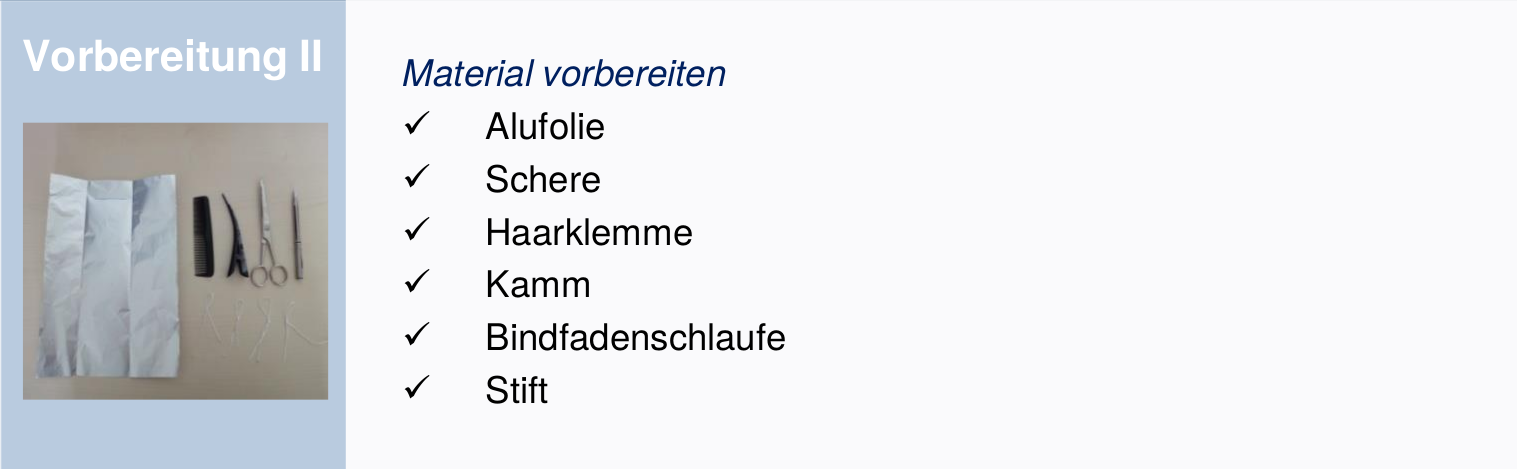
\includegraphics[width=\textwidth]{./media/SOP_Haarprobe_Entnahme_2.png}
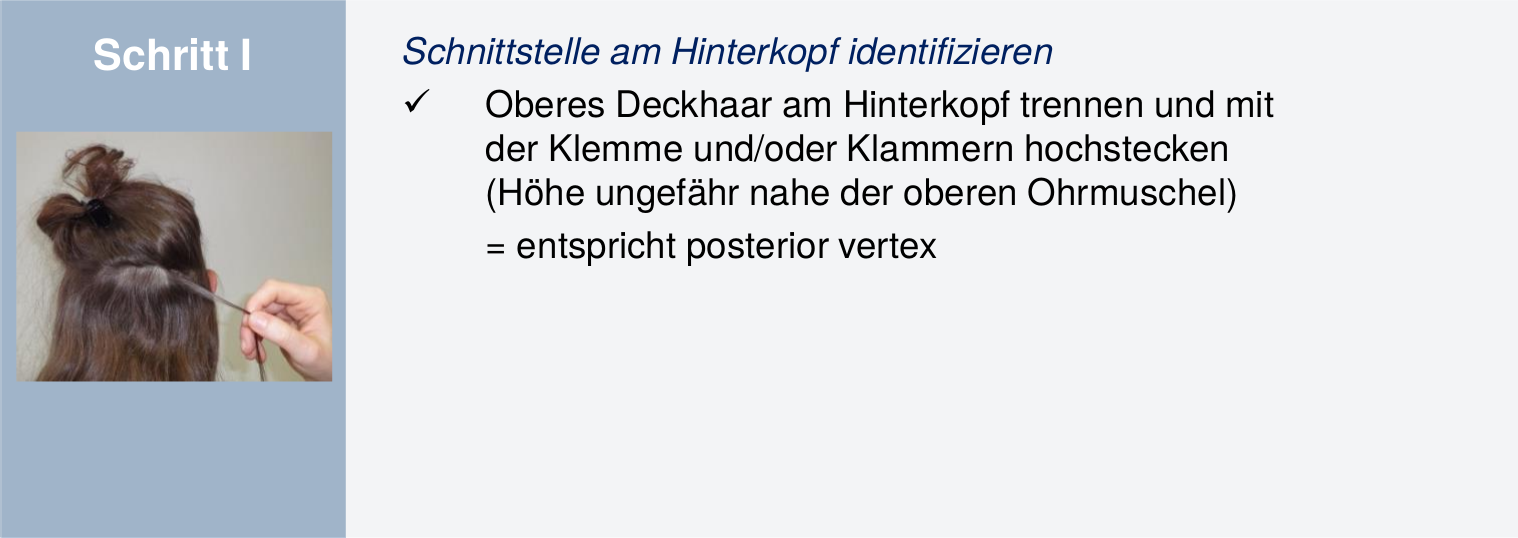
\includegraphics[width=\textwidth]{./media/SOP_Haarprobe_Entnahme_3.png}
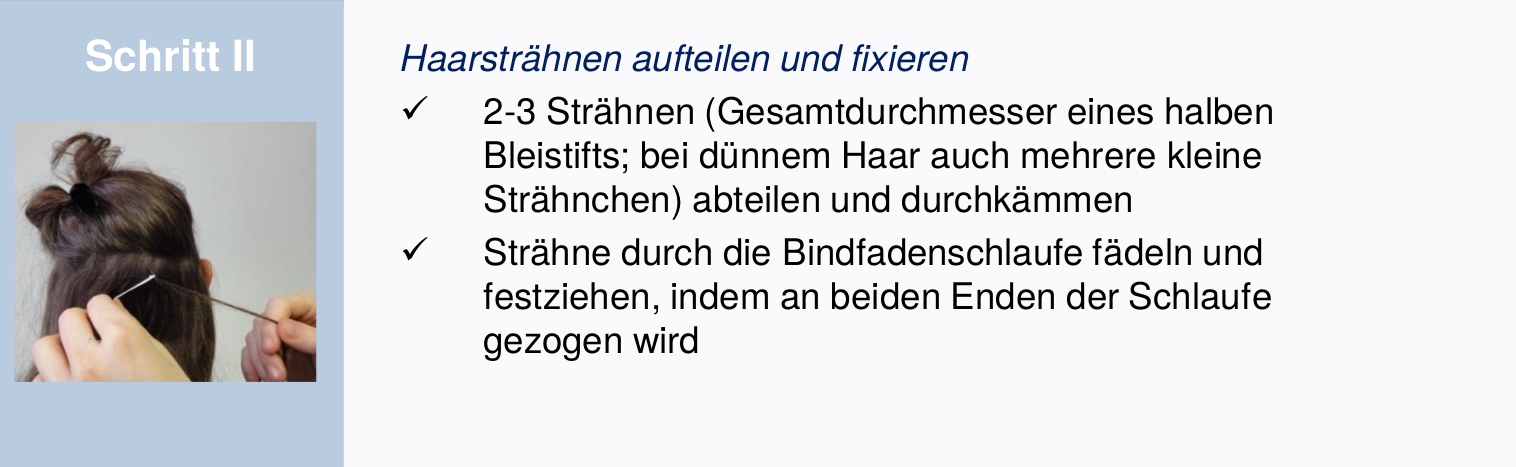
\includegraphics[width=\textwidth]{./media/SOP_Haarprobe_Entnahme_4.png}
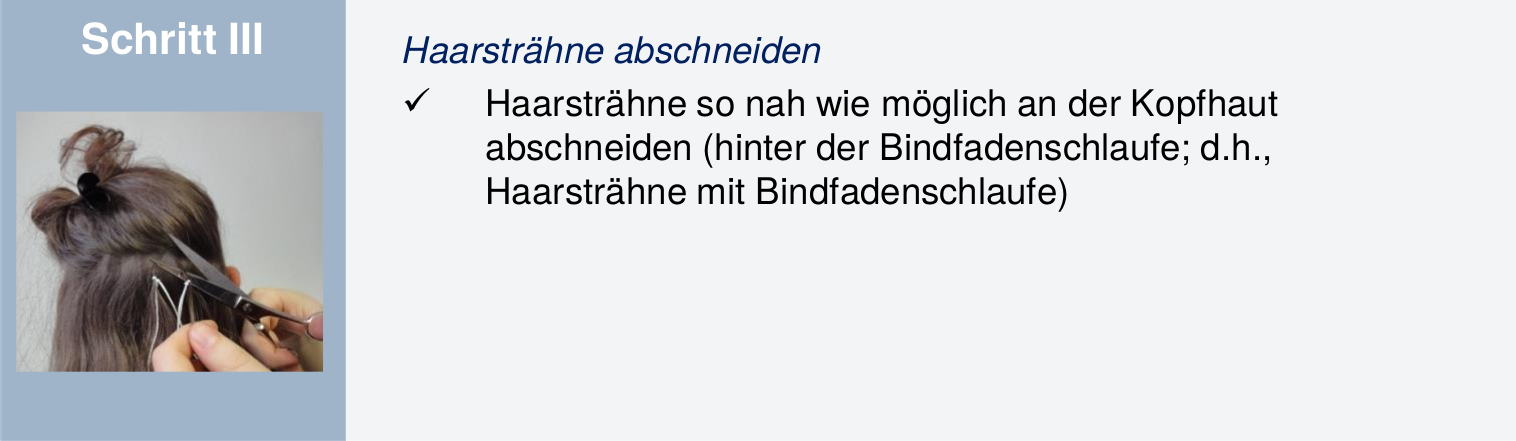
\includegraphics[width=\textwidth]{./media/SOP_Haarprobe_Entnahme_5.png}
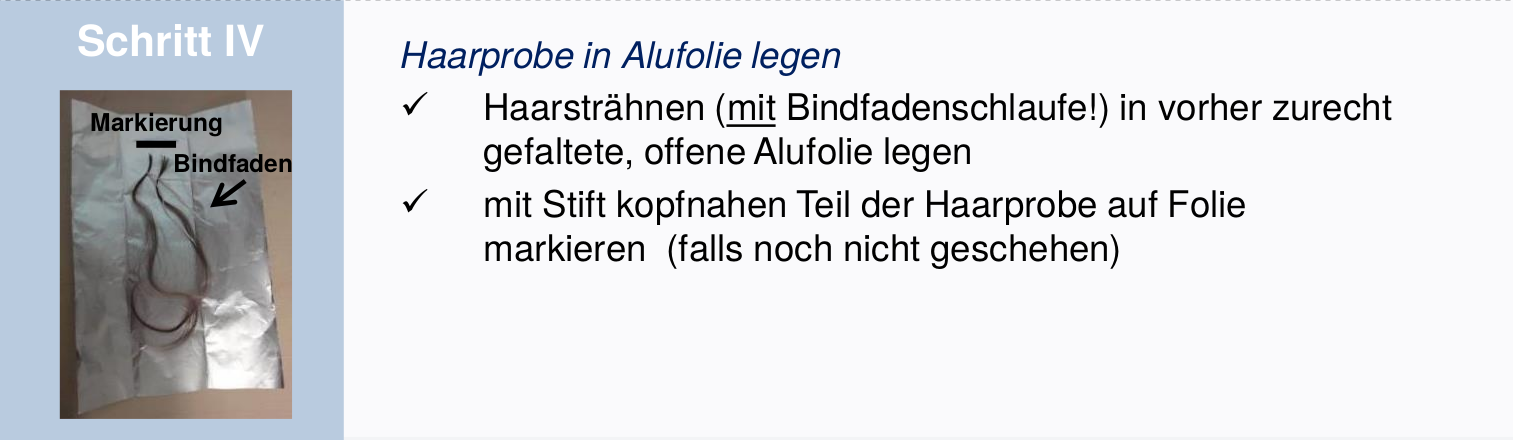
\includegraphics[width=\textwidth]{./media/SOP_Haarprobe_Entnahme_6.png}
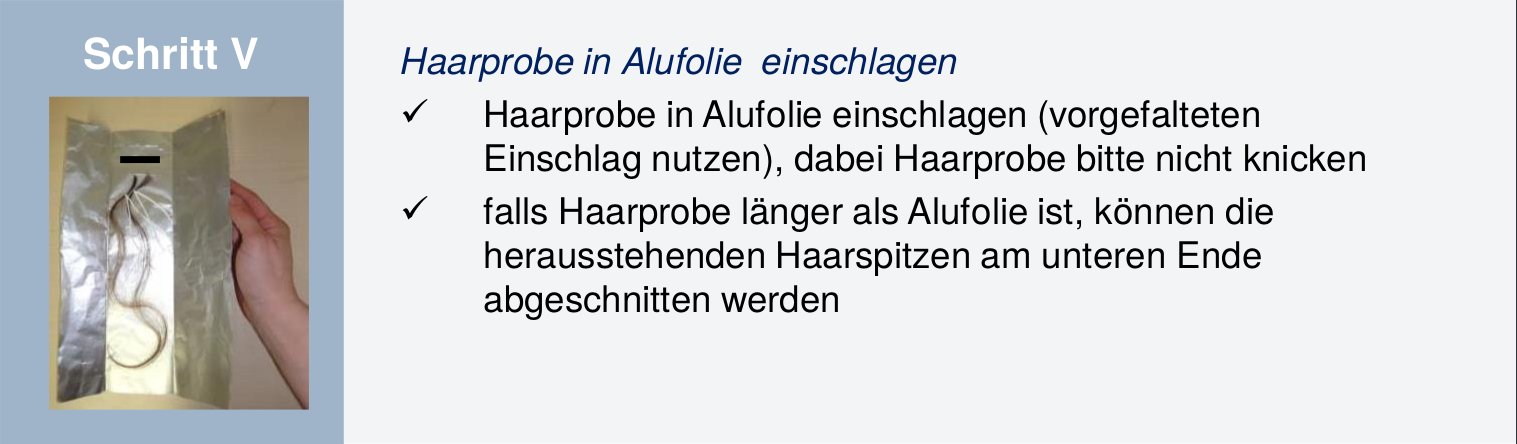
\includegraphics[width=\textwidth]{./media/SOP_Haarprobe_Entnahme_7.png}
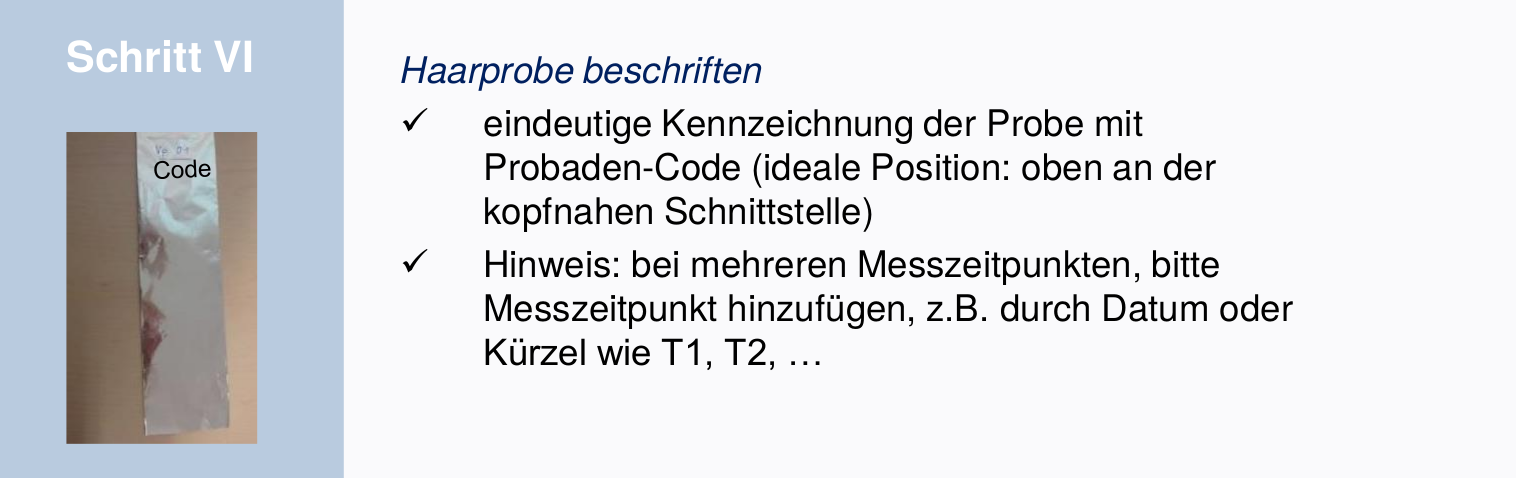
\includegraphics[width=\textwidth]{./media/SOP_Haarprobe_Entnahme_8.png}
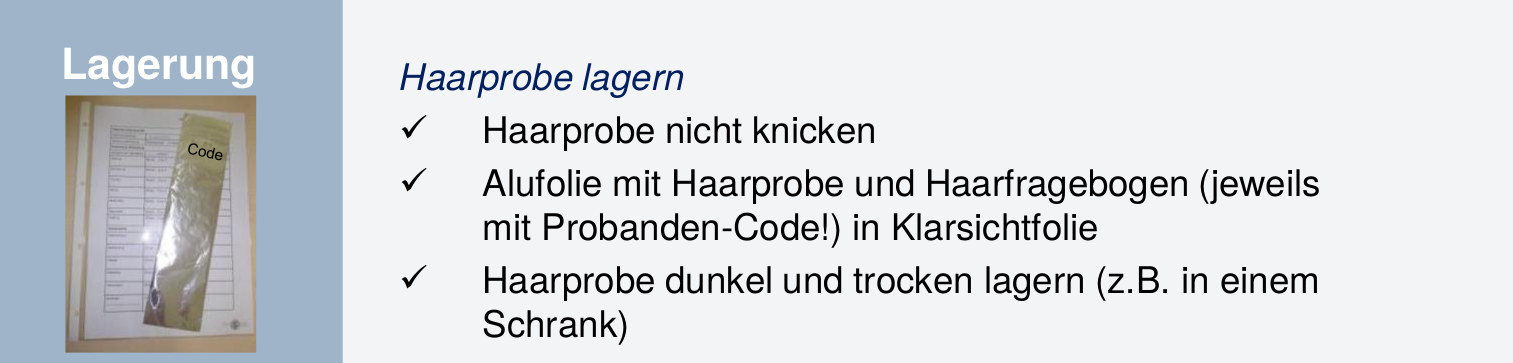
\includegraphics[width=\textwidth]{./media/SOP_Haarprobe_Entnahme_9.png}
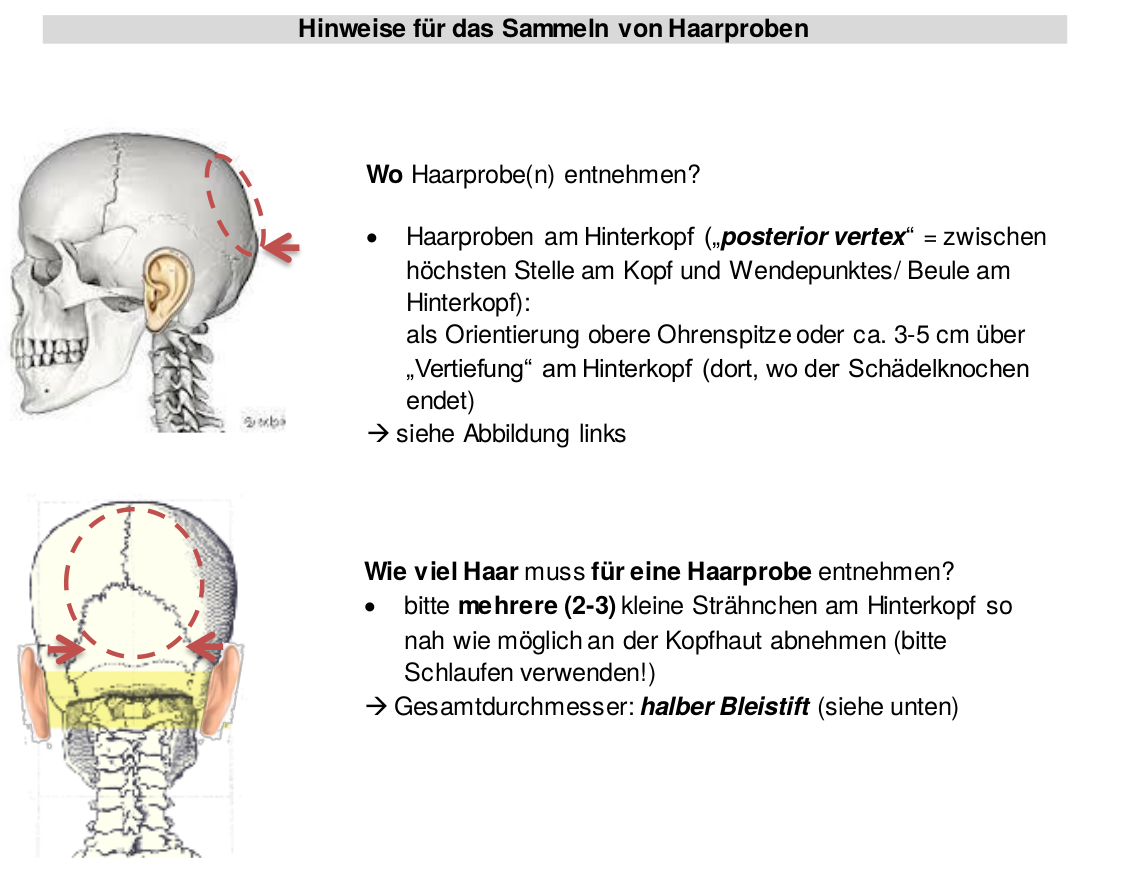
\includegraphics[width=\textwidth]{./media/SOP_Haarprobe_Hinweise_1.png}
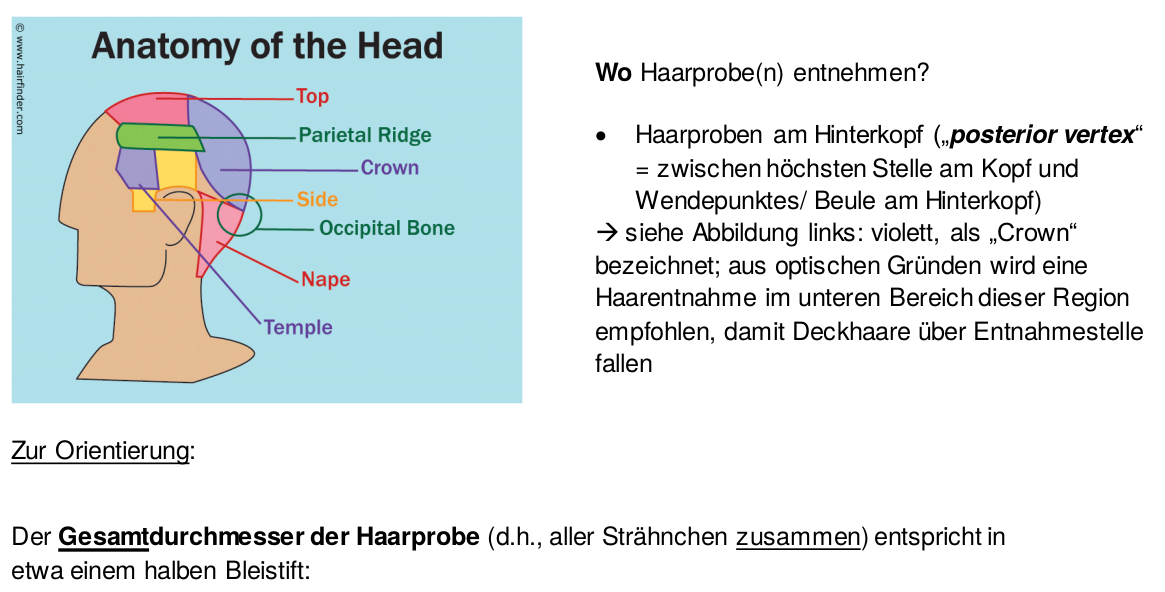
\includegraphics[width=\textwidth]{./media/SOP_Haarprobe_Hinweise_2.png}
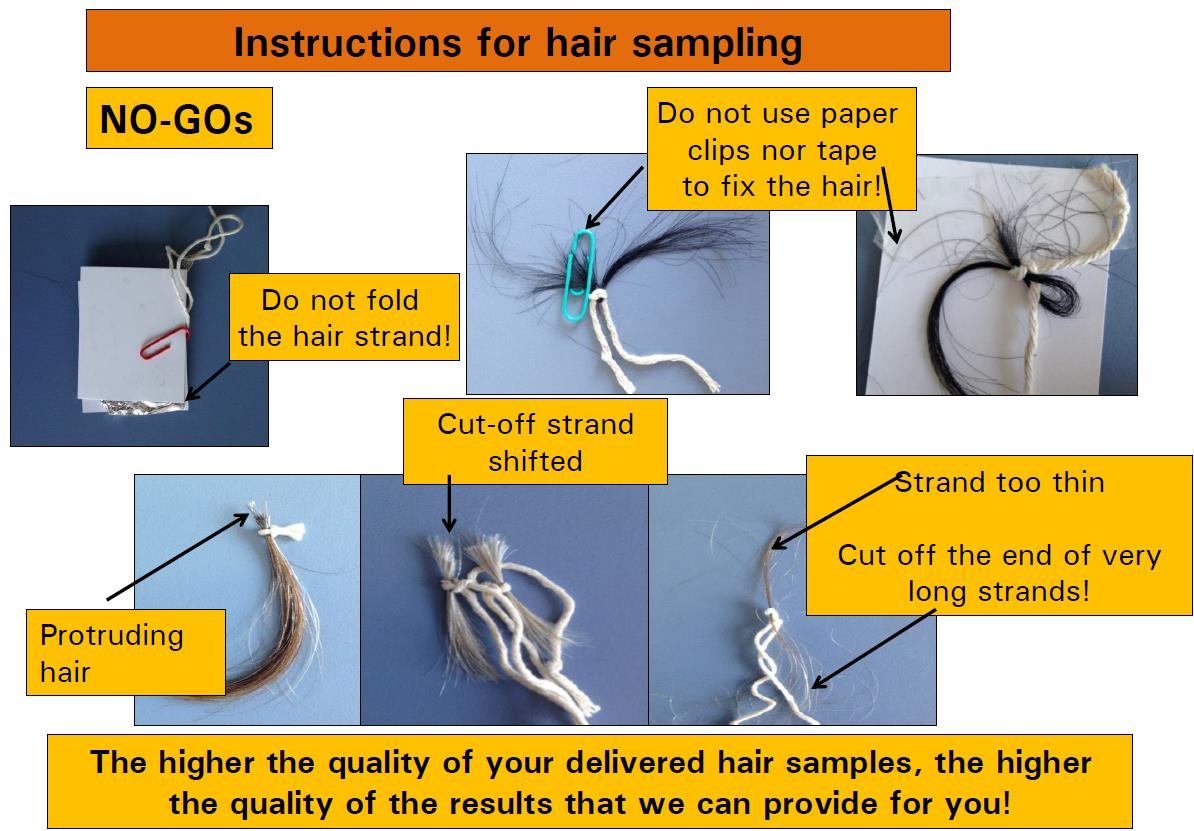
\includegraphics[width=\textwidth]{./media/SOP_Haarprobe_NoGos.png}




  \begin{center}
  {\Huge SOP Biobank -- Hessenkohorte 2040}
  
  Version 1.1 vom 17.07.2022 
\end{center}

\vspace*{1cm}

\begin{tabular}{@{}p{0.4\textwidth}l}
  erstellt von: Urs Kleinholdermann & am 17.07.2022 \\
  geprüft von: & am \\
  freigegeben von: & am \\
\end{tabular}

\vspace*{2cm}

\noindent{\Large\textbf{1. Ziel und Zweck}}

Beschreibung der Probensammlung und des down-stream-processings in der Biobank im Rahmen der longitudinalen Hessenkohorte Morbus Parkinson. \\


\noindent{\Large\textbf{2. Verbrauchsmaterial}}
\begin{itemize}
  \item Blutentnahme 	
    \begin{itemize}
      \item 1 X 4,6 ml EDTA (Blutbild)
      \item 2 x 9ml EDTA Sarstedt K2 ref. 02.1333.001 
      \item 1 x 8ml CPT (Sodium Citrate) ref. BD 362782
      \item 1 x PAXgene ref. BD 762165
      \item 1 x 15ml Falcon tube konisch 
      \item10 x 1 ml Fluid X tubes 96 ref. Brooks 68-1001-11 
    \end{itemize}
  \item Mittelstrahlurin
    \begin{itemize}
      \item 1 x 20ml urine sample 
      \item 2 x 10ml conical tube Sarstedt
      \item 20 x 1 ml Fluid X tubes 96 ref. Brooks 68-1001-11
    \end{itemize}
  \item Speichel
    \begin{itemize}
      \item 1 x Invitek 1035212200 SalivaGene Collection Module II
      \item 1 x Salivette Sarstedt Art.-Nr. 51.1534.500
    \end{itemize}
\end{itemize}

\noindent{\Large\textbf{3. Ablauf vor der Visite}}
\begin{itemize}
  \item \textbf{Checkliste:}
    Die Biobank stellt eine Checkliste bereit, die als Laufzettel für
    jede Probenahme diese in der Klinik für die Biobank dokumentiert.
  \item \textbf{Wochenplan:}
    Die Klinik sendet vor Wochenbeginn einen Probeneinsendungsplan per
    E-Mail an die Biobank. Änderungen werden per-Mail oder Telephon
    mitgeteilt.
  \item \textbf{Materialkontrolle:}
    Das Studienteam prüft wöchentlich den Materialbestand fordert bei
    Bedarf rechtzeitig entsprechende Materialien an.
\end{itemize}

\noindent{\Large\textbf{4. Probenentnahme}}
\begin{itemize}
  \item \textbf{Blut}
    \begin{itemize}
      \item Material:
        \begin{itemize}
          \item 1 X 4,6 ml EDTA Blutbild
          \item 2 x 9 ml EDTA DNA-Extraktion
          \item 1 x 8 ml CPT PBMC/Buffy Coat
          \item 1 x PAXgene	Transcriptomics
        \end{itemize}
      \item Die Blutentnahme soll in der oben angegebenen Reihenfolge
        vorgenommen werden.
      \item \textbf{Achtung!} Alle Proben werden umgehend in das
        Biobanklabor Klinikgebäude Ebene -3/ Raum 43290 transportiert
        und dort weiterverarbeitet. Der Eingang der Proben wird auf
        der Checkliste vermerkt.
      \item Die EDTA-Probe zu 4,6 ml wird in das Zentrallabor zur
        Bestimmung des Blutbildes transportiert.
      \item Wichtig ist die Berücksichtigung der Begleitschreiben von
        PAXgene sowie CPT Gefäße.
    \end{itemize}
  \item \textbf{Urin}
    \begin{itemize}
      \item 2 x 10 ml Urinröhrchen
    \end{itemize}
  \item \textbf{Speichel}
    \begin{itemize}
      \item 2 x Salivette
      \item 1 x SalivaGene Collection Module II
    \end{itemize}
\end{itemize}

\noindent{\Large\textbf{5. Prä-analytisches Liquid Handling in der Biobank}}
\begin{itemize}
  \item \textbf{3 x 9 ml EDTA}
    \begin{itemize}
      \item Die beiden Röhrchen werden zur Extraktion von DNA zu einem
        späteren Zeitpunkt eingesetzt. Das Vollblut wird in 5 ml
        Aliquots in die entsprechenden Sekundärröhrchen pipettiert und
        diese bei $-80^{\circ}C$ gelagert. Die DNA-Extraktion erfolgt zu einem
        späteren Zeitpunkt (max. Lagerzeit 12Mon.) im Institut für
        Humangenetik, Marburg.
      \item Das dritte Röhrchen dient der Plasmagewinnung und wird
        entsprechend der SOP Plasma-CBBMR prozessiert.
      \item Abweichungen werden dokumentiert.
    \end{itemize}
  \item \textbf{1 x CPT}
    \begin{itemize}
      \item Das CPT-Röhrchen dient der Gewinnung von PBMC aus Buffy
        Coat und wird nach der SOP CPT-CBBMR prozessiert. Bei Einsatz
        einer anderen Isolationsmethode für PMBC kann statt der
        CPT-Röhrchen auch ein EDTA-K2-Röhrchen zur Blutentnahme
        verwendet werden.
    \end{itemize}
  \item \textbf{PAX-Gene}
    \begin{itemize}
      \item Das PAX-Gene-Röhrchen dient der stabilisierten Gewinnung
        von RNA zur Transkriptomanalyse und wird entsprechend der SOP
        CPT-CBBMR behandelt.
    \end{itemize}
  \item \textbf{Mittelstrahlurin}
    \begin{itemize}
      \item Der Patient wird gebeten, ml frischen Mittelstrahlurin im
        ausgegebenen Behälter bereitzustellen.
      \item Noch in der Klinik wird die Probe auf Eis gelagert und in
        das Biobanklabor transportiert. Dort werden 20 ml des
        gekühlten Urins abgenommen, in 2 x 10 ml Starstedt-Urintubes
        überführt und bei 400g, $+4^{\circ}C$, 5min, ohne Bremse zentrifugiert.
      \item Die Überstände in Aliquots á 0,5 ml in entsprechende
        FluidX-Röhrchen aliquotiert und bei $-80^{\circ}C$ gelagert.
      \item Die Pellets werden in je 1,250 ml RNA-Cell Protect-Medium
        aufgenommen. und bei $-80^{\circ}C$ gelagert.
    \end{itemize}
  \item \textbf{Speichelsammlung für die Metabolomics}
    \begin{itemize}
      \item Die Sammlung des Speichels erfolgt mittels der Salivette
        (Sarstedt) zur Sammlung von unstimulated whole-mouth saliva
        (UWMS). Es werden zwei Röhrchen befüllt. Die Entnahme mittels
        “Kagummi erfolgt nach Beilagenvorschrift. Sobald das Röhrchen
        gefüllt ist, wird es auf Eis zur weiteren Laborbearbeitung
        gelagert.
      \item Das Röhrchen wir nach Vorgabe samt Kaugummi zentrifugiert
        (1200g; $+4^{\circ}C$, 20 min. ohne Bremse).
      \item Nach der Zentrifugation wird das Kaugummi entnommen und
        verworfen, die verbliebene Flüssigkeit mit der Pipette
        homogenisiert
      \item Aus der homogenisierten Flüssigkeit werden Aliquots zu je
        $150\mu l$ entnommen und bei $-80^{\circ}C$ gelagert.
   \end{itemize}
  \item \textbf{Speichelsammlung mittels SalivaGene Collection Module II für die DNA-Extraktion}
    \begin{itemize}
      \item Die Sammlung des Speichels erfolgt mittels der Saliva Gene
        Collector-Röhrchen nach Herstellerangaben. Es wird zwei
        Röhrchen befüllt. Das Röhrchen wird dicht verschlossen (bitte
        kontrollieren) und vorsichtig über Kopf für ca. 8
        Sek. geschüttelt.
      \item Das gesamte Röhrchen wird in der Biobank bei $-80^{\circ}C$ gelagert.
      \item \textbf{Achtung!} Die maximale Lagerzeit bis zur DNA-Extraktion
        sollte 12 Mon nicht überschreiten.
    \end{itemize}
\end{itemize}    




  \begin{center}
  {\Huge SOP Blutbild -- Hessenkohorte 2040}
  
  Version 1.1 vom 17.07.2022 
\end{center}

\vspace*{1cm}

\begin{tabular}{@{}p{0.4\textwidth}l}
  erstellt von: Urs Kleinholdermann & am 17.07.2022 \\
  geprüft von: & am \\
  freigegeben von: & am \\
\end{tabular}

\vspace*{2cm}

\begin{center}
  {\huge Hessenkohorte 2040 Stud.Nr. 252 Institut für
    Laboratoriumsmedizin und Pathobiochemie}
\end{center}


\begin{enumerate}
  \item Parameter: Hämatologie: kleines Blutbild
  \item Abnahmeröhrchen: EDTA –Blut
  \item Formular immer mit der Angabe der Studiennummer 252 (für
    HK2040), ausgefüllt im Zentrallabor abgeben. Formulare unter
    ISF29.3
  \item Für Fragen steht der EDV – Beauftragten des Labors Herrn
    Patrick Junk zur Verfügung • Email: Patrick.Junk@uk-gm.de Tel.:
    66535
  \item Herrn Junk über die Anzahl der benötigten Laborzettel
    informieren und den Drucker (umrdr8335) nennen, auf dem die
    Laborergebnisse nach der Auswertung gesandt werden sollen
  \item Akkreditierungsurkunde und aktuelle Ringzertifikate der
    Parameter bei Fr. Pfeifer (leitende LMTA) im Zentrallabor
    anfordern: Email: \url{doris.pfeifer@uk-gm.de} Tel.: 64468
  \item Referenzwerte der Parameter im Intranet ausdrucken (Im
    Intranet unter \emph{Institut für Laboratoriumsmedizin} --
    \emph{Leistungsverzeichnis})
  \item Nach der Beendigung der Studie werden die Kosten mit dem Labor
    abgerechnet (Kostenberechnung : 3,5 Euro pro Blutbild – s. Mail
    Prof. Stief 02.06.21)
\end{enumerate}

\end{document}
